\documentclass[journal]{IEEEtran}

\usepackage[T1]{fontenc}
\usepackage{newtxtext}
\usepackage{amsmath,amssymb,amsfonts,amsthm,mathtools,bm}
\usepackage{graphicx}
\usepackage{booktabs,tabularx,multirow,array,makecell}
\usepackage{enumitem}
\usepackage{xcolor}
\usepackage{cite}
\usepackage[colorlinks=true,linkcolor=blue!70!black,citecolor=blue!70!black,urlcolor=blue!70!black]{hyperref}

\newtheorem{theorem}{Theorem}
\newtheorem{proposition}{Proposition}
\newtheorem{lemma}{Lemma}
\newtheorem{corollary}{Corollary}
\newtheorem{assumption}{Assumption}
\newtheorem{definition}{Definition}
\newtheorem{remark}{Remark}

\setlist[enumerate]{leftmargin=1.6em,itemsep=1pt,topsep=2pt,parsep=0pt}
\setlist[itemize]{leftmargin=1.4em,itemsep=1pt,topsep=2pt,parsep=0pt}

\newcommand{\bp}{\boldsymbol{p}}
\newcommand{\bu}{\boldsymbol{u}}
\newcommand{\bg}{\boldsymbol{g}}
\newcommand{\be}{\boldsymbol{e}}
\newcommand{\br}{\boldsymbol{r}}
\newcommand{\bL}{\boldsymbol{L}_{\mathrm{p}}}
\newcommand{\bQ}{\boldsymbol{Q}_\perp}
\newcommand{\bH}{\boldsymbol{H}}
\newcommand{\bJ}{\boldsymbol{J}}
\newcommand{\I}{\boldsymbol{I}}
\newcommand{\lr}{\lambda_{\mathrm{req}}}
\newcommand{\ds}{d_{\mathrm{safe}}}
\newcommand{\norm}[1]{\lVert#1\rVert}
\newcommand{\ip}[2]{\langle#1,#2\rangle}
\newcommand{\diag}{\operatorname{diag}}
\newcommand{\col}{\operatorname{col}}
\newcommand{\clip}{\operatorname{clip}}
\newcommand{\tr}{\operatorname{tr}}

\renewcommand{\topfraction}{0.95}
\renewcommand{\bottomfraction}{0.90}
\renewcommand{\dbltopfraction}{0.95}
\renewcommand{\textfraction}{0.04}
\renewcommand{\floatpagefraction}{0.88}
\renewcommand{\dblfloatpagefraction}{0.88}
\setlength{\dblfloatsep}{8pt plus 2pt minus 2pt}
\setlength{\dbltextfloatsep}{10pt plus 2pt minus 2pt}
\setcounter{topnumber}{3}
\setcounter{dbltopnumber}{3}
\setcounter{totalnumber}{4}

\allowdisplaybreaks[1]

\begin{document}

\title{Envelope Equivariant Graph Reinforcement Learning and Neighborhood Proximal Allocation for Cooperative Deadlock Resolution of Multi-Robot Systems Under Coupled Safety Constraints}

\author{Wei~Tan and Xin~Chen,~\IEEEmembership{Member,~IEEE}%
\thanks{Manuscript received November 9, 2026. This work was supported by the National Natural Science Foundation of China. \textit{(Corresponding author: Xin Chen.)}}%
\thanks{The authors are with the School of Artificial Intelligence and Automation, China University of Geosciences, Wuhan 430074, China, and also with the Hubei Key Laboratory of Advanced Control and Intelligent Automation for Complex Systems, Wuhan 430074, China (e-mail: tanwei@cug.edu.cn; chenxin@cug.edu.cn).}%
}

\markboth{IEEE TRANSACTIONS ON ROBOTICS / AUTOMATIC CONTROL (MANUSCRIPT)}{TAN AND CHEN: ENVELOPE EQUIVARIANT GRAPH RL AND NEIGHBORHOOD PROXIMAL ALLOCATION FOR DEADLOCK RESOLUTION}

\maketitle

\begin{abstract}
Multi-robot systems operating under coupled inter-robot collision avoidance and global algebraic connectivity maintenance constraints frequently suffer from non-target geometric deadlocks in dense symmetric encounters, channel blockage by outer stationary target-holding neighbors, and terminal steady-state hovering induced by learned zero-order repulsive residuals. This paper proposes an Envelope Equivariant Graph Policy with Neighborhood Proximal Allocation (EGP-NPA) cooperative control framework. First, we construct an exact rational second-order Karush--Kuhn--Tucker (KKT) certificate on a seven-robot symmetric contact configuration, proving algebraically that even when all robots are freely mobile and an explicit collision-free, spectrally connected path exists, any myopic Control Barrier Function (CBF) safety filter enforcing monotone task-error descent ($\dot{W}\le 0$) is trapped by a positive-definite Lagrangian Hessian over the entire critical cone and a finite-radius quadratic energy barrier. This certificate identifies two necessary and sufficient physical conditions for deadlock resolution: lateral symmetry-breaking nominal drive from swapping robots and dynamic quota-driven yielding from outer stationary neighbors. Second, we construct a planar $\mathrm{SO}(2)$ rotation-, translation-, and permutation-equivariant one-hop message-passing Graph Neural Network (GNN) residual nominal policy, proving the structural necessity of chiral rotational bias over full $\mathrm{O}(2)$ reflection equivariance. Coupled with a closed-neighborhood block NPA safety shield with antisymmetric edge-ledger local settlement, we derive the explicit positive closed-form solution for pairwise quota transfer and stationary neighbor yielding velocity on contact boundaries, and prove why penalizing normal filter intervention suppresses cooperative yielding. Furthermore, a stateless one-hop closed-neighborhood completion envelope is proposed to suppress zero-order pairwise repulsive biases to $\mathcal{O}(\lVert\boldsymbol{e}_k\rVert_2)$ near the goal and restore the zero-velocity target equilibrium. Finally, trained via Multi-Agent Proximal Policy Optimization (MAPPO) on small teams ($N\in\{6,\dots,10\}, B=2$) and deployed zero-shot to larger teams ($N\in\{12,20,25\}, B=8$), EGP-NPA achieves $100\%$ safe arrival and zero safety violations across $96$ dense triangular-lattice swap/permutation benchmarks and $48$ independent holdout instances, outperforming shield-consistent safe MARL ($53.1\%$), decentralized static-CBF shielded GNN ($3.1\%$), primal-dual MAPPO-Lagrangian ($0\%$ violation-free arrival), tangential circulation heuristics ($40.6\%$), and myopic CBF filtering ($15.6\%$). Controlled fixed-weight ablations and second-order \texttt{MuJoCo} virtual-physical simulations with online division-free spectral estimation further validate each module and characterize the safety-margin versus channel-passability trade-off.
\end{abstract}

\begin{IEEEkeywords}
Multi-robot systems, control barrier functions, algebraic connectivity, safe reinforcement learning, equivariant graph neural networks, geometric deadlock, neighborhood proximal allocation.
\end{IEEEkeywords}

\section{Introduction}\label{sec:intro}

\IEEEPARstart{I}{n} cooperative inspection, on-demand wireless communication relaying, and dense formation reconfiguration, multi-robot systems must simultaneously avoid inter-robot collisions and maintain the global connectivity of state-dependent communication graphs so that distributed estimation and decision-making pipelines remain unbroken \cite{yang2010decentralized,sabattini2013decentralized,ong2021connectivity}. Control Barrier Functions (CBFs) \cite{ames2017cbf,breeden2022sampled} provide a computationally efficient Quadratic Program (QP) safety filtering paradigm by translating forward invariance of a safe set into affine inequality constraints on the control input. For multi-agent systems subject to coupled safety constraints comprising pairwise collision avoidance and a global Laplacian algebraic connectivity lower bound, recent advances in nonsmooth spectral barrier functions \cite{ong2021connectivity}, continuous-time violation-free distributed gradient flows \cite{tan2025violationfree}, and zero-sum Neighborhood Proximal Allocation (NPA) allow robots to compute strictly safe control inputs at each sampling instant using only a finite number of one-hop neighbor communication rounds.

However, instantaneous single-step feasibility of a safety filter does not imply long-horizon task completion. When multiple robots encounter one another in narrow passages or must exchange positions inside a tightly packed array, nominal attractive velocities pointing toward individual goals are frequently canceled by normal reaction forces from active collision and connectivity constraints, trapping the system permanently in non-target symmetric equilibria (i.e., geometric deadlocks) \cite{reis2021,grover2023deadlock,tan2024equilibria,mestres2026filters}. From a convex-optimization and physical perspective, traditional minimally invasive CBF filters lock up in dense encounters due to their myopic structure that enforces step-by-step monotone descent of the raw position error $W(\bp)=\frac12\sum_{i=1}^N\norm{\bp_i-\bg_i}_2^2$. Projecting the negative-gradient nominal velocity $-k_g\nabla_{\bp}W=-k_g(\bp-\bg)$ onto a safe input set containing the zero-velocity vector necessarily enforces $\dot W(\bp(t))\le 0$ \cite{allibhoy2024safegradient}. In dense formations where interior robots must swap positions while outer neighbors already reside at their respective goals ($\bp_j=\bg_j$), this monotonicity requirement induces a dual lock-up: first, the radial goal attraction of the swapping robots is collinearly canceled by the direct contact normal force; second, any temporary outward movement of a stationary outer neighbor to open a geometric passage momentarily increases $W(\bp)$, and under static equal quota splitting its local feasible set collapses to a singleton at zero velocity on the contact boundary \cite{karagoz2014navigation}.

To mitigate spurious equilibria and deadlocks in safety filters, two primary lines of research have been pursued: analytical circulation heuristics and learning-based safe control. On the analytical side, Reis et al. \cite{reis2021} and Tan and Dimarogonas \cite{tan2024equilibria} characterized undesired equilibria and saddle instabilities of CBF-QPs, while Gon\c{c}alves et al. \cite{goncalves2023circulation} and Dai et al. \cite{dai2024compatible} introduced tangential circulation terms and compatible Control Lyapunov--Barrier Functions (CLF-CBFs) to break collinear stagnation. Nevertheless, when interior swapping robots are surrounded by multiple layers of stationary target-holding neighbors, uniform constant-sign circulation triggers rotational conflicts across adjacent contact edges. More fundamentally, when a symmetric contact configuration constitutes a \emph{strict constrained local minimum} rather than an unstable saddle point, no local negative-curvature perturbation or $\dot W\le 0$ feedback can cross the surrounding energy barrier. On the learning side, primal-dual Lagrangian safe MARL (MAPPO-Lagrangian) \cite{gu2023safe}, predictive and adaptive safety-filter reinforcement learning \cite{wabersich2021,liu2026saferl}, Neural Graph CBFs (GCBF+) \cite{zhang2025gcbf}, and Discrete Graph Proximal Policy Optimization (DGPPO) \cite{zhang2025dgppo} employ Graph Neural Networks (GNNs) to learn multi-agent coordination and collision-avoidance policies. Despite their progress, existing safe Multi-Agent Reinforcement Learning (MARL) methods face three unresolved structural limitations:
\begin{enumerate}
 \item \textbf{Lack of anytime zero-violation guarantees under global spectral connectivity constraints:} Neural barrier certificates and soft penalty rewards only handle pairwise relative-state collision constraints approximately and cannot guarantee deterministic, finite-round zero-violation invariance under global Laplacian algebraic connectivity constraints $\lambda_2(\bL(\bp))\ge\lr$ and sampled-data Zero-Order Hold (ZOH) execution.
 \item \textbf{Disconnection between learned nominal policies and distributed quota allocation:} Existing safety layers typically rely on independent single-agent projections or static equal responsibility splitting ($B=0$), which freezes stationary target-holding neighbors ($\be_j=\boldsymbol 0$) and forces the nominal policy to explicitly coordinate yielding trajectories for all outer nodes, suffering from severe credit-assignment inefficiency.
 \item \textbf{Terminal steady-state hovering induced by zero-order repulsive residuals:} Pairwise relative-direction biases output by message-passing GNNs are zero-order terms that do not vanish automatically as $\be_k\to\boldsymbol 0$. On tightly packed target lattices with millimeter-scale clearance, persistent contact dual multipliers keep conflict gates open, causing steady-state limit-cycle hovering outside the goal tolerance ball.
\end{enumerate}

To overcome these limitations, this paper proposes an \emph{Envelope Equivariant Graph Policy with Neighborhood Proximal Allocation} (EGP-NPA) cooperative control architecture, which decomposes dense multi-robot deadlock resolution into three tightly coupled modules: a one-hop equivariant GNN residual nominal policy, a closed-neighborhood block dynamic quota-sharing shield, and a stateless one-hop closed-neighborhood completion envelope. The main contributions of this work are fourfold:
\begin{enumerate}
 \item \textbf{Exact Rational Second-Order KKT Certificate of a Strict Non-Target Local Minimum (Theorem~\ref{thm:seven-kkt}):} Using a rationally closed polynomial channel kernel and exact rational arithmetic ($\mathbb Q$), we construct an explicit primal--dual KKT witness on a seven-robot symmetric contact configuration where all robots are mobile. We prove that the Lagrangian Hessian is strictly positive definite over the entire critical cone ($\boldsymbol v^{\top}\boldsymbol H_L\boldsymbol v\ge\frac{19}{515}\norm{\boldsymbol v}_2^2$) and establish a finite-radius quadratic energy barrier $W(\bar\bp+\boldsymbol\delta)-W(\bar\bp)\ge\frac1{100}\norm{\boldsymbol\delta}_2^2>0$ for all collision-free perturbations $0<\norm{\boldsymbol\delta}_2\le\frac1{200}$ (which persists on an open ball $B_\rho(\bp_0)$ in the strict interior of $\mathcal S$), alongside an explicit safe, spectrally connected reachability path ($\lambda_2(\bL)\ge 1792/625>5/2$). This certificate algebraically rules out saddle-escape or monotone-descent controllers and identifies two necessary and sufficient physical conditions for deadlock resolution: lateral symmetry-breaking nominal drive from swapping robots and dynamic quota-driven yielding from stationary neighbors.
 \item \textbf{$\mathrm{SO}(2)\ltimes\mathbb R^2$ and Permutation-Equivariant One-Hop GNN Residual Nominal Policy with Chiral Symmetry Breaking (Proposition~\ref{prop:equivariance}):} We construct a parameter-shared 2-layer message-passing GNN over local target/edge orthogonal frames and compressed filter algebraic states (single-agent refit shadow prices $\boldsymbol\mu_{i,k-1}$, spectral quotas, and edge ledgers). We prove exact equivariance under planar rigid-body transformations $\mathrm{SO}(2)\ltimes\mathbb R^2$ and node permutations $S_N$, and prove both theoretically and empirically why preserving $\mathrm{SO}(2)$ chiral orientation is essential whereas enforcing full $\mathrm{O}(2)$ reflection equivariance forces tangential circulation $\omega_{i,k}^\theta\equiv 0$ on mirror-symmetric head-on configurations.
 \item \textbf{Closed-Form Cooperative Unfreezing via Dynamic Quota Transfer and One-Hop Completion Envelope Theory (Propositions~\ref{prop:safety}--\ref{prop:envelope}):} We prove anytime continuous-time hard safety invariance during noisy RL exploration and finite-round zero-shot cross-scale execution (Proposition~\ref{prop:safety}). We derive the explicit closed-form solution for pairwise quota transfer $|t_{ij}^\star|=\frac{\eta\ds}{\eta+4\ds^2}\delta_n>0$ and stationary neighbor yielding velocity $-\boldsymbol n_{ij}^{\top}\bu_j^\star=\frac{\eta}{2(\eta+4\ds^2)}\delta_n>0$ driven by a moving robot's normal intrusion $\delta_n>0$ (Proposition~\ref{prop:unfreeze}), proving why static equal splitting ($B=0$) causes artificial freezing and why penalizing normal filter intervention suppresses $\delta_n>0$. We further propose the one-hop closed-neighborhood completion envelope $\rho_{i,k}$, proving that it preserves cooperative residuals during transit while enforcing $\mathcal O(\norm{\be_k}_2)$ first-order vanishing of zero-order pairwise bias at the goal (Proposition~\ref{prop:envelope}).
 \item \textbf{Small-Scale Short-Horizon Training, Zero-Shot Cross-Scale Generalization, and Second-Order Virtual-Physical Verification:} Trained via MAPPO only on small teams ($N\in\{6,\dots,10\},B=2$), EGP-NPA achieves $96/96$ ($100\%$) arrival with $0$ step cuts and $0$ rational audit violations across $64$ training-scale ($N=8$) and $32$ zero-shot cross-scale ($N\in\{12,20,25\},B=8$) dense lattice benchmarks, plus $48/48$ on an independent holdout suite. Controlled fixed-weight ablations and second-order \texttt{MuJoCo} omnidirectional chassis simulations coupled with an online division-free spectral estimator further validate the causal role of each module and establish the physical safety-margin versus channel-passability trade-off (Theorem~\ref{thm:passability-tradeoff}).
\end{enumerate}

\emph{Notation:} $\mathbb R^n$, $\mathbb Q^n$, and $\mathbb S_+^n$ denote the $n$-dimensional real vector space, rational vector space, and $n\times n$ real symmetric positive semidefinite cone, respectively. $\I_n$ is the $n\times n$ identity matrix, $\boldsymbol 1_N\in\mathbb R^N$ is the all-ones vector, and $\boldsymbol\varepsilon_i\in\mathbb R^N$ is the $i$-th standard basis vector. $\norm{\cdot}_2$ denotes the Euclidean vector norm or spectral matrix norm; $\col(\boldsymbol x_1,\dots,\boldsymbol x_m)=[\boldsymbol x_1^{\top},\dots,\boldsymbol x_m^{\top}]^{\top}$; $\otimes$ is the Kronecker product; $(x)_+=\max(x,0)$; $\clip(x,a,b)=\min(\max(x,a),b)$; $\bJ=\begin{bmatrix}0&-1\\1&0\end{bmatrix}$ is the $90^\circ$ counterclockwise rotation matrix satisfying $\bJ^{\top}=-\bJ$ and $\bJ^2=-\I_2$; and $\mathbb I(\cdot)$ is the indicator function.

\section{Problem Formulation and Preliminaries on Closed-Neighborhood NPA}\label{sec:model}

\subsection{Planar Multi-Robot Fixed-Goal Model and Rationally Closed Channel}
Consider $N$ mobile robots operating in the Euclidean plane $\mathbb R^2$ with vertex set $\mathcal V=\{1,\dots,N\}$. Each robot $i\in\mathcal V$ obeys velocity-bounded single-integrator kinematics:
\begin{equation}
 \dot\bp_i(t)=\bu_i(t),\qquad \bu_i(t)\in\mathcal U_i:=\big\{\boldsymbol v\in\mathbb R^2:\norm{\boldsymbol v}_2\le U\big\},
 \label{eq:kinematics}
\end{equation}
where $\bp_i\in\mathbb R^2$ and $\bu_i\in\mathbb R^2$ are the planar position and velocity control input of robot $i$, and $U>0$ is the maximum speed bound ($U=0.50\ \mathrm{m/s}$ throughout this paper). Given distinct static labeled goal positions $\bg_i\in\mathbb R^2$ satisfying $\norm{\bg_i-\bg_j}_2\ge\ds$ ($\forall i\ne j$), define the stacked state $\bp=\col(\bp_1,\dots,\bp_N)\in\mathbb R^{2N}$, joint input $\bu=\col(\bu_1,\dots,\bu_N)\in\mathbb R^{2N}$, and goal configuration $\bg=\col(\bg_1,\dots,\bg_N)\in\mathbb R^{2N}$. Let $\be_i=\bp_i-\bg_i$, $\be=\bp-\bg$, $\bp_{ij}=\bp_i-\bp_j$, and $d_{ij}=\norm{\bp_{ij}}_2$. The raw navigation task distance cost is defined as
\begin{equation}
 W(\bp)=\frac12\norm{\be}_2^2=\frac12\sum_{i=1}^N\norm{\bp_i-\bg_i}_2^2.
 \label{eq:W-def}
\end{equation}

To rigorously separate intrinsic geometric deadlocks of the mathematical model from floating-point rounding artifacts during equilibrium certification and sampled-data ZOH verification, the physical communication graph employs a polynomial squared-cutoff channel kernel that is algebraically closed over the rational field $\mathbb Q$:
\begin{equation}
 \omega(d)=\left(1-\frac{d^2}{R_c^2}\right)_+^2,\qquad R_c=10.0\ \mathrm m.
 \label{eq:poly-channel}
\end{equation}
Within the communication support $d<R_c$, the edge weight $w_{ij}(\bp)=\omega(d_{ij})$ is a quadratic polynomial in the squared distance $d_{ij}^2=\norm{\bp_i-\bp_j}_2^2$, continuously differentiable at $d=R_c$ with locally Lipschitz gradient. With incidence vector $\boldsymbol b_{ij}=\boldsymbol\varepsilon_i-\boldsymbol\varepsilon_j\in\mathbb R^N$, the state-dependent weighted graph Laplacian is
\begin{equation}
 \bL(\bp)=\sum_{1\le i<j\le N}\omega(d_{ij})\boldsymbol b_{ij}\boldsymbol b_{ij}^{\top}\in\mathbb S_+^N.
 \label{eq:laplacian}
\end{equation}
Whenever $\bp\in\mathbb Q^{2N}$, $\bL(\bp)$ and all its directional derivatives are exact rational matrices, enabling zero-error verification of KKT optimality conditions and matrix positive definiteness via exact rational arithmetic.

\subsection{Composite Safe Set and Sampled-Data ZOH Segment Safety}
Let $0=\lambda_1(\bL(\bp))\le\lambda_2(\bL(\bp))\le\cdots\le\lambda_N(\bL(\bp))$ denote the ordered eigenvalues of $\bL(\bp)$, where $\lambda_2(\bL(\bp))$ is the algebraic connectivity. The composite safe configuration set is $\mathcal S:=\mathcal X\cap\mathcal C$, where $\mathcal X=[-B_{\mathrm{ws}},B_{\mathrm{ws}}]^{2N}$ is the bounded workspace and
\begin{equation}
 \mathcal C=\big\{\bp\in\mathbb R^{2N}:\ d_{ij}\ge\ds\ (\forall i<j),\ \lambda_2(\bL(\bp))\ge\lr\big\}
 \label{eq:safe-set}
\end{equation}
enforces both pairwise collision avoidance $\ds>0$ and global algebraic connectivity maintenance $\lr>0$.

Choosing an orthogonal complement basis matrix $\bQ\in\mathbb R^{N\times(N-1)}$ satisfying $\bQ^{\top}\bQ=\I_{N-1}$ and $\bQ^{\top}\boldsymbol 1_N=\boldsymbol 0$, the compressed spectral margin matrix on the zero-mean subspace is defined as
\begin{equation}
\begin{split}
 \bH(\bp)&=\bQ^{\top}\bL(\bp)\bQ-\lr\I_{N-1},\\
 \bH(\bp)&\succeq\boldsymbol 0\ \Longleftrightarrow\ \lambda_2(\bL(\bp))\ge\lr.
\end{split}\label{eq:H-matrix}
\end{equation}
Its directional derivative along $\bu$ is $D\bH(\bp)[\bu]=\bQ^{\top}\sum_{i<j}[\nabla_{\bp_i}w_{ij}^{\top}(\bu_i-\bu_j)]\boldsymbol b_{ij}\boldsymbol b_{ij}^{\top}\bQ$. With pairwise barrier function $h_{ij}^{\mathrm{col}}(\bp)=d_{ij}^2-\ds^2$ and barrier decay rates $\alpha_c,\alpha_s,\alpha_x>0$, the continuous-time composite safe input set is
\begin{equation}
\begin{split}
 \mathcal K_0(\bp)&=\Big\{\bu\in\mathbb R^{2N}:\ 2\bp_{ij}^{\top}(\bu_i-\bu_j)+\alpha_c h_{ij}^{\mathrm{col}}(\bp)\ge 0,\\
 &\quad D\bH(\bp)[\bu]+\alpha_s\bH(\bp)\succeq\boldsymbol 0,\\
 &\quad \bu_i\in\mathcal U_i,\ |p_{i,a}+\alpha_x^{-1}u_{i,a}|\le B_{\mathrm{ws}}\ (\forall i<j,\,a)\Big\}.
\end{split}\label{eq:K0-def}
\end{equation}
For every $\bp\in\mathcal S$, $\mathcal K_0(\bp)$ is nonempty, closed, and convex, and always contains the zero-velocity vector $\boldsymbol 0\in\mathcal K_0(\bp)$. Given a nominal velocity $\bu^{\mathrm{nom}}\in\mathbb R^{2N}$, the centralized minimally invasive safety projection is
\begin{equation}
 \Pi_{\mathcal K_0(\bp)}(\bu^{\mathrm{nom}})=\arg\min_{\bu\in\mathcal K_0(\bp)}\frac12\norm{\bu-\bu^{\mathrm{nom}}}_2^2.
 \label{eq:central-proj}
\end{equation}

Under sampled-data ZOH execution at $t_k=k\Delta t$ ($\Delta t=0.05\ \mathrm s$), the executed velocity $\bu_k$ is held constant over $[t_k,t_k+h]$, generating the straight-line segment $\bp(s)=\bp_k+s\bu_k$ ($s\in[0,h]$). Using the explicit second-order curvature bound $\frac{\mathrm d^2}{\mathrm ds^2}\bH(\bp_k+s\bu_k)\succeq -c_L\norm{\bu_k}_2^2\I_{N-1}$ with $c_L=8N/R_c^2$ for the polynomial kernel \eqref{eq:poly-channel}, we obtain the following continuous-time segment safety guarantee.

\begin{theorem}[Continuous-Time Safety Over ZOH Segments]\label{thm:zoh-safe}
Suppose $\bp_k\in\mathcal S$ and step size $h>0$ satisfies $\alpha_c h\le 1,\alpha_s h\le 1,\alpha_x h\le 1$. If $\bu_k$ satisfies the speed ball, workspace bounds, pairwise collision CBF inequalities in \eqref{eq:K0-def}, and the curvature-tightened spectral condition
\begin{equation}
 D\bH(\bp_k)[\bu_k]+\alpha_s\bH(\bp_k)\succeq\frac{c_L h}{2}\norm{\bu_k}_2^2\I_{N-1},
 \label{eq:zoh-tightened}
\end{equation}
then the continuous trajectory $\bp(s)=\bp_k+s\bu_k$ satisfies $d_{ij}(s)\ge\ds$ ($\forall i<j$), $\lambda_2(\bL(\bp(s)))\ge\lr$, and $\bp(s)\in\mathcal X$ for all $s\in[0,h]$.
\end{theorem}
\begin{proof}
For each pair $i<j$, exact quadratic expansion of $h_{ij}^{\mathrm{col}}(\bp_k+s\bu_k)$ together with \eqref{eq:K0-def} and $\alpha_c s\le 1$ yields
\begin{equation}
\begin{split}
 h_{ij}^{\mathrm{col}}(\bp_k+s\bu_k)&=h_{ij}^{\mathrm{col}}(\bp_k)+2s\bp_{ij,k}^{\top}(\bu_{i,k}-\bu_{j,k})\\
 &\quad+s^2\norm{\bu_{i,k}-\bu_{j,k}}_2^2\\
 &\ge(1-\alpha_c s)h_{ij}^{\mathrm{col}}(\bp_k)\ge 0.
\end{split}
\end{equation}
For $\bH(\bp_k+s\bu_k)$, second-order Taylor expansion with integral remainder and \eqref{eq:zoh-tightened} yield, for all $s\in[0,h]$,
\begin{equation}
\begin{split}
 \bH(\bp_k+s\bu_k)&\succeq\bH(\bp_k)+sD\bH(\bp_k)[\bu_k]\\
 &\quad-\tfrac12 c_L s^2\norm{\bu_k}_2^2\I_{N-1}\\
 &\succeq(1-\alpha_s s)\bH(\bp_k)\\
 &\quad+\tfrac12 c_L s(h-s)\norm{\bu_k}_2^2\I_{N-1}\succeq\boldsymbol 0.
\end{split}
\end{equation}
Workspace bounds hold for all $s\in[0,h]$ by convexity.
\end{proof}

\subsection{Closed-Neighborhood Block NPA and Antisymmetric Edge-Ledger Settlement}\label{subsec:npa-prelim}
At step $k$, the linearized coupled safety constraints are written as $M_k=1+P_k$ affine inequality rows:
\begin{equation}
 \sum_{i\in\mathcal V_a}\big(\boldsymbol a_{ia,k}^{\top}\bu_i+b_{ia,k}\big)\le 0,\qquad a\in\{0,1,\dots,P_k\},
 \label{eq:coupled-rows}
\end{equation}
where row $a=0$ ($\mathcal V_0=\mathcal V$) is the Fiedler spectral connectivity row with unit Fiedler eigenvector $\boldsymbol\phi_k$ ($\boldsymbol 1_N^{\top}\boldsymbol\phi_k=0,\norm{\boldsymbol\phi_k}_2=1$) and discretization margin $\delta_\lambda>0$ ($\lambda_{\mathrm{eff}}=\lr+\delta_\lambda$), i.e., $\boldsymbol a_{i0,k}=-\sum_{j\ne i}(\phi_{i,k}-\phi_{j,k})^2\nabla_{\bp_i}w_{ij}(\bp_k)$ and $b_{i0,k}=-\frac{\alpha_s}{N}(\lambda_2(\bL(\bp_k))-\lambda_{\mathrm{eff}})$; rows $a\in\{1,\dots,P_k\}$ ($\mathcal V_a=\{i,j\}$) are pairwise collision rows with $\boldsymbol a_{ia,k}=-2\bp_{ij,k},\boldsymbol a_{ja,k}=2\bp_{ij,k}$, and $b_{ia,k}=b_{ja,k}=-\frac{\alpha_c}{2}(d_{ij,k}^2-\ds^2)$. Note that $b_{ia,k}\le 0$ holds throughout $\mathcal S$ (the zero-velocity feasible initialization condition). In dense triangular-lattice interior swap tasks, robots permute locally within the compact lattice without global expansion, so $\lambda_2(\bL(\bp(t)))\gg\lr$ (e.g., $\lambda_2\approx 15.3\gg\lr=9.69$ in Section~\ref{sec:experiments}) and the active geometric bottleneck arises from tightly coupled pairwise contact constraints at $\ds=1.000\ \mathrm m$.

Over the one-hop directed communication graph $\mathcal G_{\mathrm c}(\bp_k)=(\mathcal V,\mathcal E_k)$ defined by sensing/communication radius $R_{\mathrm{sense}}=2.50\ \mathrm m$ (open neighborhood $\mathcal N_{i,k}=\{j:0<d_{ij,k}\le R_{\mathrm{sense}}\}$, closed neighborhood $\mathcal N_{i,k}^+=\{i\}\cup\mathcal N_{i,k}$), each robot maintains zero-sum quota variables $s_{ia,k}$ reconstructed from antisymmetric edge ledgers $\varpi_{e,a,k}$ on undirected edges $e=\{i,j\}$:
\begin{equation}
 s_{ia,k}=\sum_{e\ni i}\sigma_{i,e}\varpi_{e,a,k}\ \Longrightarrow\ \sum_{i\in\mathcal V_a}s_{ia,k}=0,
 \label{eq:edge-ledger}
\end{equation}
where $\sigma_{i,e}=+1,\sigma_{j,e}=-1$ for $i<j$. The closed-neighborhood NPA safety filter $L$ executes two stages per control step:
\begin{enumerate}
 \item \textbf{Stage 1 (Link-loss revocation, single-robot safety refit, and one-hop local settlement):} Edges exceeding $R_{\mathrm{sense}}$ have their ledgers zeroed by both endpoints. Each robot $i\in\mathcal V$ then solves the local refit QP under inherited quotas $\boldsymbol s_{i,k-1}$ (with nonnegative KKT multiplier vector $\boldsymbol\mu_{i,k-1}$):
 \begin{equation}
 \begin{split}
  \min_{\bu_i\in\mathcal U_i\cap\mathcal X_i}&\ \frac12\norm{\bu_i-\bu_{i,k}^{\mathrm{nom}}}_2^2\\
  \text{s.t.}\quad&\ \boldsymbol a_{ia,k}^{\top}\bu_i+b_{ia,k}+s_{ia,k-1}\le 0,\ \forall a\ni i.
 \end{split}\label{eq:refit-one}
 \end{equation}
 If \eqref{eq:refit-one} is infeasible for robot $i$, one-hop local settlement clears all incident edge ledgers of node $i$ ($s_{ia}=0$, restoring feasibility of $\bu_i=\boldsymbol 0$ since $b_{ia,k}\le 0$) and notifies one-hop neighbors to re-solve \eqref{eq:refit-one}, yielding a strictly feasible warm start $(\bu_k^{(0)},\boldsymbol s_k^{(0)})$.
 \item \textbf{Stage 2 ($B$-round closed-neighborhood block proximal allocation):} In round $r\in\{1,\dots,B\}$, each closed-neighborhood induced subgraph $\mathcal G_i^+=(\mathcal N_{i,k}^+,E_i)$ solves in parallel:
 \begin{equation}
 \begin{split}
  \min_{\tilde\bu_q,w_q,t_e}&\ \frac12\!\sum_{q\in\mathcal N_{i,k}^+}\!\norm{\tilde\bu_q-\bu_{q,k}^{\mathrm{nom}}}_2^2\\
  &\quad+\frac{1}{2\eta}\!\sum_{q\in\mathcal N_{i,k}^+}\!w_q^2+\frac{1}{\eta}\!\sum_{e\in E_i}\!t_e^2\\
  \text{s.t.}\ &\ \boldsymbol a_{q0,k}^{\top}\tilde\bu_q+b_{q0,k}+s_{q0,k}^{(r-1)}+w_q\le 0,\\
  &\ \boldsymbol a_{qa,k}^{\top}\tilde\bu_q+b_{qa,k}+s_{qa,k}^{(r-1)}+\!\sum_{e\in E_{i,a}}\!\sigma_{q,e}t_e\le 0,\\
  &\ \sum_{q\in\mathcal N_{i,k}^+}w_q=0,\quad \tilde\bu_q\in\mathcal U_q\cap\mathcal X_q,
 \end{split}\label{eq:block-qp}
 \end{equation}
 where $\eta=2.0$ is the proximal parameter, $w_q$ is the block spectral quota increment, and $t_e$ is the pairwise collision quota transfer on edge $e\in E_{i,a}=\{e\in E_i:a(e)=a\}$. Block solutions are committed via convex combination weights $\vartheta_i=(\max_{q\in\mathcal N_{i,k}^+}|\mathcal N_{q,k}^+|)^{-1}$:
 \begin{equation}
  \bu_q^{(r)}=\Big(1-\sum_{i:q\in\mathcal N_{i,k}^+}\vartheta_i\Big)\bu_q^{(r-1)}+\sum_{i:q\in\mathcal N_{i,k}^+}\vartheta_i\tilde\bu_q^{(i)}.
  \label{eq:convex-commit}
 \end{equation}
\end{enumerate}

\section{Obstruction of Myopic Error-Monotone Control and Rational KKT Certificate}\label{sec:obstruction}

\subsection{Variational Inequality and Normal-Cone Lock-Up of Myopic Projections}
In standard safety-critical navigation \cite{ames2017cbf,reis2021}, each robot uses the proportional goal-attraction nominal law $\bu_i^{\mathrm{nom}}=-k_g\be_i=-k_g(\bp_i-\bg_i)$ ($k_g>0$), yielding the filtered input $\bu_G=\Pi_{\mathcal K_0(\bp)}(-k_g\be)$. By the variational inequality of Euclidean projection onto the closed convex set $\mathcal K_0(\bp)$,
\begin{equation}
 (\bu_G+k_g\be)^{\top}(\boldsymbol v-\bu_G)\ge 0,\qquad\forall\boldsymbol v\in\mathcal K_0(\bp).
 \label{eq:vi-proj}
\end{equation}
Substituting the always-safe zero velocity $\boldsymbol v=\boldsymbol 0\in\mathcal K_0(\bp)$ into \eqref{eq:vi-proj} yields
\begin{equation}
 \dot W(\bp)=\be^{\top}\bu_G\le -\frac{1}{k_g}\norm{\bu_G}_2^2\le 0.
 \label{eq:W-descent}
\end{equation}
Equation~\eqref{eq:W-descent} shows that whenever $\boldsymbol 0\in\mathcal K_0(\bp)$, any proportional-attraction safety filter enforces monotone nonincreasing $W(\bp(t))$. However, at a non-target configuration ($\be\ne\boldsymbol 0$), if $-k_g\be$ falls into the normal cone $N_{\mathcal K_0(\bp)}(\boldsymbol 0)=\{\boldsymbol w\in\mathbb R^{2N}:\boldsymbol w^{\top}\boldsymbol v\le 0,\ \forall\boldsymbol v\in\mathcal K_0(\bp)\}$ \cite{rockafellar1970}, no nonzero safe velocity can decrease $W$ to first order, and the unique global optimum of the safety QP collapses to $\bu_G=\boldsymbol 0$.

\subsection{Seven-Robot Strict Non-Target Local Minimum Theorem and Energy Barrier}\label{subsec:seven-kkt}
Deadlocks in CBF filters are often treated as unstable saddle points escapable via small perturbations or negative curvature \cite{reis2021,tan2024equilibria}. To rigorously falsify the universality of this assumption when all robots are mobile, consider the seven-robot planar symmetric double-triangle configuration $\bar\bp\in\mathbb R^{14}$ shown in Fig.~\ref{fig:seven-geom}(a) ($\ds=1\ \mathrm m,U=1/2\ \mathrm{m/s}$, columns correspond to robots $1,\dots,7$):
\begin{equation}
 \bar\bp^{\top}=\begin{bmatrix}
 -1 & -1/2 & -1/2 & 0 & 1/2 & 1/2 & 1\\
 0 & \sqrt{3}/2 & -\sqrt{3}/2 & 0 & \sqrt{3}/2 & -\sqrt{3}/2 & 0
 \end{bmatrix}.
 \label{eq:seven-config}
\end{equation}
At $\bar\bp$, all $7$ robots are mobile and form $12$ active contact edges at $d_{ij}=1\ \mathrm m$: $\mathcal E_c=\{12,13,14,24,25,34,36,45,46,47,57,67\}$. Outer robots $1,2,3,5,6$ start at their respective goals ($\bg_i=\bar\bp_i,\be_i=\boldsymbol 0$), whereas center robot $4$ at $(0,0)$ and rightmost robot $7$ at $(1,0)$ must exchange positions ($\bg_4=\bar\bp_7,\bg_7=\bar\bp_4$).

\begin{figure*}[htbp]
 \centering
 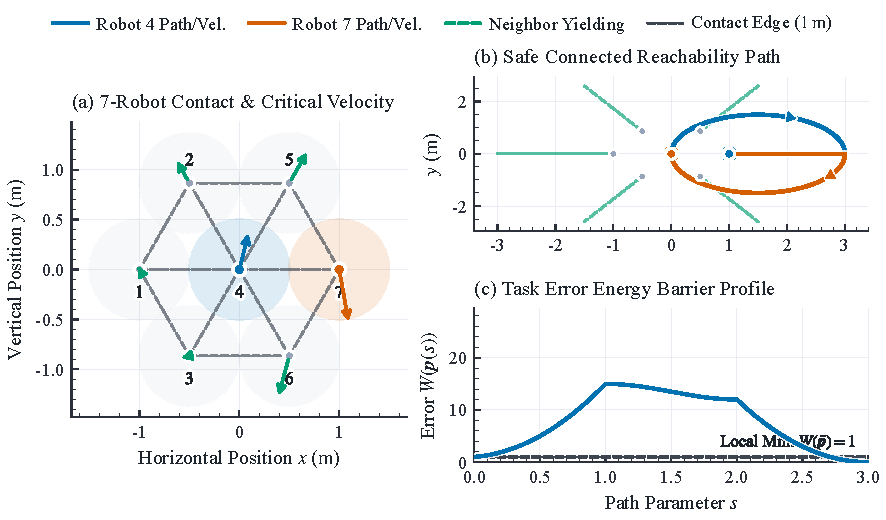
\includegraphics[width=\textwidth]{figures_en/fig1_seven_geometry.pdf}
 \caption{Seven-robot strict non-target local minimum configuration and analytical safe connected reachability witness. (a) Double-triangle contact configuration \eqref{eq:seven-config}, $12$ initial contact edges, and optimal critical-cone velocity witness vectors \eqref{eq:certificate-primal}; (b) analytical 3-stage reachability path (uniform expansion by $3$, opposite semicircular swap of robots $4$ and $7$, and uniform contraction); (c) task error profile $W(\bp(s))$ along the witness path, illustrating the mandatory energy barrier above $W(\bar\bp)=1$.}
 \label{fig:seven-geom}
\end{figure*}

\begin{theorem}[Exact Rational Certificate of Strict Local Minimum and Energy Barrier]\label{thm:seven-kkt}
For the seven-robot position swap task \eqref{eq:seven-config} with $\ds=1\ \mathrm m,\lr=5/2,R_c=10\ \mathrm m$:
\begin{enumerate}
 \item \textbf{First-order stationarity and second-order strict positive definiteness on the critical cone:} At $\bar\bp$, $W(\bar\bp)=1$, $\lambda_2(\bL(\bar\bp))>5/2$, and $\nabla W(\bar\bp)=\frac12\nabla h_{47}^{\mathrm{col}}(\bar\bp)$, so $\bu_G=\boldsymbol 0$ is the unique optimum of \eqref{eq:central-proj}. Over the full critical cone $\mathcal C=\{\boldsymbol v\in\mathbb R^{14}:\bar\bp_{ij}^{\top}(\boldsymbol v_i-\boldsymbol v_j)\ge 0\ (\forall\{i,j\}\in\mathcal E_c),\ v_{4x}=v_{7x}\}$, the Lagrangian Hessian $\boldsymbol H_L=\I_{14}-(\boldsymbol b_{47}\boldsymbol b_{47}^{\top})\otimes\I_2$ satisfies the exact rational bounds:
 \begin{equation}
 \begin{split}
  \min_{\boldsymbol v\in\mathcal C,\ v_{4y}-v_{7y}=1}\norm{\boldsymbol v}_2^2&=\frac{515}{496}>1,\\
  \boldsymbol v^{\top}\boldsymbol H_L\boldsymbol v&\ge\frac{19}{515}\norm{\boldsymbol v}_2^2>0\quad(\forall\boldsymbol v\in\mathcal C\setminus\{\boldsymbol 0\}).
 \end{split}\label{eq:critical-hessian}
 \end{equation}
 \item \textbf{Finite-radius spherical energy barrier and strictly interior open-ball trap:} For every collision-free perturbation $0<\norm{\boldsymbol\delta}_2\le\frac1{200}$ satisfying $d_{ij}(\bar\bp+\boldsymbol\delta)\ge 1$ ($\forall i<j$),
 \begin{equation}
  W(\bar\bp+\boldsymbol\delta)-W(\bar\bp)\ge\frac{1}{100}\norm{\boldsymbol\delta}_2^2>0.
  \label{eq:finite-barrier}
 \end{equation}
 Moreover, for the strictly interior perturbed task $\bp_0=(1+10^{-8})\bar\bp,\bg_\tau=(1+10^{-6})\bg$, every continuous safe trajectory starting in the open ball $B_\rho(\bp_0)\subset\operatorname{int}(\mathcal S)$ of radius $\rho=\frac{1}{4\times 10^8}$ with $\dot W_\tau\le 0$ is permanently trapped inside the sphere $\norm{\bp-\bar\bp}_2=\frac1{200}$ ($W_\tau(\bar\bp+\boldsymbol\delta)-W_\tau(\bar\bp)\ge\frac{19}{8\times 10^7}>W_\tau(\bp)-W_\tau(\bar\bp)$) and cannot reach the exterior goal $\bg_\tau$.
 \item \textbf{Global collision-free and spectrally connected reachability:} There exists an explicit piecewise smooth path $\bp(s)$ ($s\in[0,3]$) connecting the initial and goal configurations such that $d_{ij}(s)\ge 1\ \mathrm m$ and $\lambda_2(\bL(\bp(s)))\ge\frac{1792}{625}=2.8672>\frac52$ for all $s\in[0,3]$.
\end{enumerate}
\end{theorem}
\begin{proof}
(1) At $\bar\bp$, $\be_4=(-1,0)^{\top},\be_7=(1,0)^{\top}$, and $\be_i=\boldsymbol 0$ otherwise, while $\nabla_{\bp_4}h_{47}^{\mathrm{col}}(\bar\bp)=(-2,0)^{\top}$ and $\nabla_{\bp_7}h_{47}^{\mathrm{col}}(\bar\bp)=(2,0)^{\top}$; thus multiplier $\lambda_{47}=1/2$ (and $0$ on all other edges) satisfies $\nabla W(\bar\bp)-\frac12\nabla h_{47}^{\mathrm{col}}(\bar\bp)=\boldsymbol 0$. For $\boldsymbol v\in\mathcal C$, $\boldsymbol v^{\top}\boldsymbol H_L\boldsymbol v=\norm{\boldsymbol v}_2^2-|v_{4y}-v_{7y}|^2$. Scaling coordinates as $\boldsymbol v_i=(z_{ix},\sqrt{3}z_{iy})^{\top}$ stacked into $\boldsymbol z\in\mathbb R^{14}$ with $Q_c=\diag(1,3,\dots,1,3)$ gives $\norm{\boldsymbol v}_2^2=\boldsymbol z^{\top}Q_c\boldsymbol z$. Define rational matrices $(G_c\boldsymbol z)_{ij}=\bar p_{ij,x}(z_{ix}-z_{jx})+\sqrt{3}\bar p_{ij,y}(z_{iy}-z_{jy})$ and $E_c\boldsymbol z=[z_{4x}-z_{7x},\,z_{4y}-z_{7y}]^{\top}$. For the convex QP $\min\boldsymbol z^{\top}Q_c\boldsymbol z\ \text{s.t.}\ G_c\boldsymbol z\ge\boldsymbol 0,\,E_c\boldsymbol z=(0,1)^{\top}$, the exact rational primal witness $Z_*\in\mathbb Q^{7\times 2}$ and dual multipliers $(\boldsymbol\mu,\boldsymbol\nu)$ are:
\begin{equation}
\begin{split}
 Z_*^{\top}&=\frac{1}{496}{\setlength{\arraycolsep}{2.5pt}\begin{bmatrix}
 -15 & -132 & -105 & 90 & 177 & -105 & 90\\
 15 & 132 & -15 & 206 & 177 & -225 & -290
 \end{bmatrix}},\\
 \mu_{13}&=\tfrac{15}{248},\ \mu_{24}=\tfrac{33}{62},\ \mu_{36}=\tfrac{15}{62},\ \mu_{45}=\tfrac{177}{248},\ \mu_{67}=\tfrac{225}{248},\\
 \boldsymbol\nu&=\big[\tfrac{135}{496},\,\tfrac{1545}{496}\big]^{\top},
\end{split}\label{eq:certificate-primal}
\end{equation}
with all other $\mu_{ij}=0$. Exact rational arithmetic verifies primal feasibility $G_c\boldsymbol z_*\ge\boldsymbol 0,E_c\boldsymbol z_*=(0,1)^{\top}$, complementary slackness $\boldsymbol\mu^{\top}G_c\boldsymbol z_*=0$, and stationarity $Q_c\boldsymbol z_*=G_c^{\top}\boldsymbol\mu+E_c^{\top}\boldsymbol\nu$, with optimal objective $\boldsymbol z_*^{\top}Q_c\boldsymbol z_*=\frac{1545}{496}$. Dividing by the vertical scaling factor $3$ yields $\min_{\boldsymbol v\in\mathcal C,v_{4y}-v_{7y}=1}\norm{\boldsymbol v}_2^2=\frac{515}{496}>1$ and $\boldsymbol v^{\top}\boldsymbol H_L\boldsymbol v\ge(1-\frac{496}{515})\norm{\boldsymbol v}_2^2=\frac{19}{515}\norm{\boldsymbol v}_2^2$.

(2) Let $0<R:=\norm{\boldsymbol\delta}_2\le\frac1{200}$ satisfy $\norm{\bar\bp_{ij}+\boldsymbol\delta_i-\boldsymbol\delta_j}_2^2\ge 1$ ($\forall\{i,j\}\in\mathcal E_c$). With $z=\delta_{4x}-\delta_{7x}$ and $t=\delta_{4y}-\delta_{7y}$, we have $W(\bar\bp+\boldsymbol\delta)-W(\bar\bp)=\frac12 R^2-z$. If $z\le 0$, \eqref{eq:finite-barrier} holds trivially; suppose $z>0$. Each contact edge gives $\bar\bp_{ij}^{\top}(\boldsymbol\delta_i-\boldsymbol\delta_j)\ge -\frac12\norm{\boldsymbol\delta_i-\boldsymbol\delta_j}_2^2\ge -R^2$. Taking the inner product of $Q_c\boldsymbol z_*=G_c^{\top}\boldsymbol\mu+E_c^{\top}\boldsymbol\nu$ with the scaled perturbation $\tilde{\boldsymbol\delta}$, using $\sum\mu_{ij}=\frac{609}{248}=:S$, $c=\frac{1545}{496}$, and the Cauchy--Schwarz inequality gives $\frac{c}{\sqrt{3}}|t|\le\sqrt{c}R+SR^2\implies t^2\le\frac{496}{515}R^2(1+\frac32 R)^2$. Moreover, $(-1+z)^2+t^2\ge 1\implies 2z\le z^2+t^2$ and $z\le 2R^2$, whence
\begin{equation}
\begin{split}
 W(\bar\bp+\boldsymbol\delta)-W(\bar\bp)&=\frac12 R^2-z\\
 &\ge\frac{R^2}{2}\left[1-\frac{496}{515}\Big(1+\frac32 R\Big)^2-4R^2\right]\\
 &\ge\frac{1}{100}R^2,\qquad\forall R\in\Big(0,\frac1{200}\Big].
\end{split}
\end{equation}
The strictly interior trap on $B_\rho(\bp_0)$ follows from $W_\tau(\bar\bp+\boldsymbol\delta)-W_\tau(\bar\bp)\ge\frac{r^2}{100}-\frac52\tau r=\frac{19}{8\times 10^7}$ on $\norm{\boldsymbol\delta}_2=r=\frac1{200}$.

(3) Along the 3-stage path in Fig.~\ref{fig:seven-geom}(b) (uniform expansion to $3\bar\bp$, opposite semicircular swap of robots $4$ and $7$ around $(3/2,0)$ with radius $3/2$, and uniform contraction to $\bg$), all pairwise distances satisfy $d_{ij}(s)\ge 1$ and $\max_{i<j}d_{ij}(s)\le 6$, so $w_{ij}(s)\ge(1-36/100)^2=256/625$ and $\lambda_2(\bL(\bp(s)))\ge 7\times\frac{256}{625}=\frac{1792}{625}>\frac52$.
\end{proof}

\begin{remark}[Two Necessary and Sufficient Physical Conditions for Deadlock Resolution]\label{rem:two-conditions}
The exact rational witness \eqref{eq:certificate-primal} establishes two fundamental physical conditions required to unlock dense interior swaps:
\begin{enumerate}
 \item \textbf{Lateral symmetry-breaking nominal drive from swapping robots:} In \eqref{eq:certificate-primal}, robots $4$ and $7$ must generate opposite transverse velocity components $z_{4y}=+\frac{206}{496}>0$ and $z_{7y}=-\frac{290}{496}<0$ perpendicular to $\be_4,\be_7$. Purely radial attraction keeps the system inside the collinear deadlock subspace $v_{4y}-v_{7y}=0$.
 \item \textbf{Cooperative yielding of outer stationary neighbors via dynamic quota transfer:} As robots $4$ and $7$ separate transversely, the five outer target-holding neighbors ($\be_j=\boldsymbol 0$) must simultaneously execute nonzero outward yielding velocities (e.g., $(Z_*)_{2,:}=\frac1{496}[-132,132]$, $(Z_*)_{5,:}=\frac1{496}[177,177]$), transmitted mechanically through strictly positive contact shadow prices $\mu_{24},\mu_{45},\mu_{67}>0$. Under static equal quota splitting ($s_{ia}\equiv 0$), stationary neighbors remain frozen at $\bu_j=\boldsymbol 0$ and truncate the transverse separation of robots $4$ and $7$ to zero.
\end{enumerate}
\end{remark}

\section{Envelope Equivariant Graph Policy with Neighborhood Proximal Allocation (EGP-NPA)}\label{sec:method}

\subsection{Chiral Rotation- and Permutation-Equivariant One-Hop GNN Residual Nominal Policy}\label{subsec:gnn-arch}
To break the collinear deadlock identified in Remark~\ref{rem:two-conditions} without hand-crafting global topological potentials, we construct a distributed residual nominal policy over the one-hop directed communication graph $\mathcal G_{\mathrm c}(\bp_k)=(\mathcal V,\mathcal E_k)$ at $t_k=k\Delta t$ ($R_{\mathrm{sense}}=2.50\ \mathrm m$).

Feeding raw Cartesian coordinates $\bp_{i,k},\bg_i$ into a neural network violates Euclidean rigid-body invariance, causing identical relative formations rotated or translated in the workspace to produce inconsistent actions \cite{satorras2021egnn}. For each robot $i\in\mathcal V$, we construct a local target orthonormal frame using $\hat{\be}_{i,k}=\be_{i,k}/\max(\norm{\be_{i,k}}_2,10^{-9})$ and $\bJ\hat{\be}_{i,k}$, together with a smooth goal-vanishing factor $\sigma_{i,k}=\min(1,\norm{\be_{i,k}}_2/r_0)$ ($r_0=0.10\ \mathrm m$) to remove directional singularity as $\be_{i,k}\to\boldsymbol 0$. For each directed edge $(i,j)\in\mathcal E_k$, we construct a local edge orthonormal frame using $\hat{\br}_{ij,k}=(\bp_{j,k}-\bp_{i,k})/d_{ij,k}$ and $\bJ\hat{\br}_{ij,k}$.

Let $\bu_{i,k-1}$ be the previous executed velocity, $\boldsymbol\delta_{i,k-1}=\bu_{i,k-1}-\Pi_{\mathcal U_i}(\bu_{i,k-1}^{\mathrm{nom}})$ the filter velocity modification, $\boldsymbol\mu_{i,k-1}$ the KKT dual multiplier vector (shadow prices) from the single-robot refit QP \eqref{eq:refit-one}, $s_{i0,k-1}$ the spectral quota, and $\boldsymbol\varpi_{e,k-1}=[\varpi_{ij,0,k-1},\varpi_{ij,1,k-1}]^{\top}$ the binary edge ledger on $e=\{i,j\}$. Define the one-hop closed-neighborhood conflict memory $m_{i,k}=\max\bigl(\gamma_m m_{i,k-1},\max_{j\in\mathcal N_{i,k}^+}c_{j,k-1}\bigr)$ and gate $\gamma_{i,k}^{\mathrm{gate}}=\tanh(\beta_m m_{i,k})\in[0,1)$ ($\gamma_m=0.97,\beta_m=4.0$; $c_{j,k-1}=\norm{\boldsymbol\mu_{j,k-1}}_2$ gives the shadow-price gate $\gamma_{i,k}^{\mathrm{gate},\mu}$, while $c_{j,k-1}=\norm{\boldsymbol\delta_{j,k-1}}_2$ gives the intervention gate $\gamma_{i,k}^{\mathrm{gate,int}}$). The rotation-invariant node feature $\boldsymbol x_{i,k}=\col(\boldsymbol x_{i,k}^{\mathrm{geom}},\boldsymbol x_{i,k}^{\mathrm{alg}})\in\mathbb R^{17}$ and directed edge feature $\boldsymbol e_{ij,k}^{\mathrm{feat}}=\col(\boldsymbol e_{ij,k}^{\mathrm{geom}},\boldsymbol e_{ij,k}^{\mathrm{alg}})\in\mathbb R^{20}$ are constructed as:
\begin{equation}
\begin{split}
 \boldsymbol x_{i,k}^{\mathrm{geom}}&=\Big[\min(\norm{\be_{i,k}}_2,4),\ \mathbb I(\norm{\be_{i,k}}_2<\varepsilon_g),\ \gamma_{i,k}^{\mathrm{gate}},\\
 &\quad\ \tfrac{\norm{\bu_{i,k-1}}_2}{U},\ \tfrac{\bu_{i,k-1}^{\top}\hat{\be}_{i,k}}{U}\sigma_{i,k},\ \tfrac{\bu_{i,k-1}^{\top}\bJ\hat{\be}_{i,k}}{U}\sigma_{i,k},\\
 &\quad\ \tfrac{\norm{\boldsymbol\delta_{i,k-1}}_2}{U},\ \tfrac{\boldsymbol\delta_{i,k-1}^{\top}\hat{\be}_{i,k}}{U}\sigma_{i,k},\ \tfrac{\boldsymbol\delta_{i,k-1}^{\top}\bJ\hat{\be}_{i,k}}{U}\sigma_{i,k},\\
 &\quad\ \tfrac{\lambda_2(\bL(\bp_k))-\lr}{\lr},\ \tfrac{|\mathcal N_{i,k}|}{8},\ \min_{j\in\mathcal N_{i,k}}(d_{ij,k}-\ds)\Big]^{\top},
\end{split}\label{eq:node-geom}
\end{equation}
\begin{equation}
\begin{split}
 \boldsymbol e_{ij,k}^{\mathrm{geom}}&=\Big[\tfrac{d_{ij,k}}{R_{\mathrm{sense}}},\ \clip(d_{ij,k}-\ds,0,1.5),\ \hat{\br}_{ij,k}^{\top}\hat{\be}_{i,k}\sigma_{i,k},\\
 &\quad\ \hat{\br}_{ij,k}^{\top}\bJ\hat{\be}_{i,k}\sigma_{i,k},\ \hat{\br}_{ij,k}^{\top}\hat{\be}_{j,k}\sigma_{j,k},\ \hat{\br}_{ij,k}^{\top}\bJ\hat{\be}_{j,k}\sigma_{j,k},\\
 &\quad\ \min(\norm{\be_{j,k}}_2,4),\ \hat{\be}_{i,k}^{\top}\hat{\be}_{j,k}\sigma_{i,k}\sigma_{j,k},\\
 &\quad\ (\bJ\hat{\be}_{i,k})^{\top}\hat{\be}_{j,k}\sigma_{i,k}\sigma_{j,k},\ \tfrac{(\bu_{j,k-1}-\bu_{i,k-1})^{\top}\hat{\br}_{ij,k}}{U},\\
 &\quad\ \tfrac{(\bu_{j,k-1}-\bu_{i,k-1})^{\top}\bJ\hat{\br}_{ij,k}}{U},\ \gamma_{j,k}^{\mathrm{gate}},\ \tfrac{\norm{\boldsymbol\delta_{j,k-1}}_2}{U}\Big]^{\top},
\end{split}\label{eq:edge-geom}
\end{equation}
\begin{equation}
\begin{split}
 \boldsymbol x_{i,k}^{\mathrm{alg}}&=\Big[\ln(1+|\mu_{i0,k-1}|),\ \ln\big(1+\textstyle\sum_{j\ne i}|\mu_{ij,k-1}|\big),\\
 &\quad\ \clip\big(\tfrac{s_{i0,k-1}}{\bar\nu_{i0,k}},-3,3\big),\ \ln(1+\norm{\boldsymbol\mu_{i,k-1}}_2),\\
 &\quad\ \clip\big(\tfrac{U\norm{\boldsymbol a_{i0,k}}_2-b_{i0,k}-s_{i0,k-1}}{\bar\nu_{i0,k}},-3,3\big)\Big]^{\top},\\
 \boldsymbol e_{ij,k}^{\mathrm{alg}}&=\Big[\ln(1+|\mu_{ij,k-1}|),\ \ln(1+|\mu_{ji,k-1}|),\\
 &\quad\ \tanh(2\varpi_{ij,0,k-1}),\ \tanh(2\varpi_{ij,1,k-1}),\\
 &\quad\ |\tilde\phi_{i,k}-\tilde\phi_{j,k}|,\ \norm{\widetilde{\boldsymbol\Phi}_{i,k}-\widetilde{\boldsymbol\Phi}_{j,k}}_2,\ \widetilde{\boldsymbol\Phi}_{i,k}^{\top}\widetilde{\boldsymbol\Phi}_{j,k}\Big]^{\top},
\end{split}\label{eq:alg-feat}
\end{equation}
where $\bar\nu_{i0,k}=U\norm{\boldsymbol a_{i0,k}}_2+|b_{i0,k}|+10^{-3}$ normalizes the spectral row, and $\tilde\phi_{i,k}=\sqrt{N}\phi_{i,k}$, $\widetilde{\boldsymbol\Phi}_{i,k}=\sqrt{N}\boldsymbol\Phi_{i,k}\in\mathbb R^2$ are unit-RMS normalized spectral states satisfying $\frac1N\sum_{i=1}^N\tilde\phi_{i,k}^2=1$.

A parameter-shared $L_{\mathrm{gnn}}=2$-layer message-passing GNN encodes $\boldsymbol h_i^{(0)}=\phi_{\mathrm{enc}}(\boldsymbol x_{i,k})\in\mathbb R^{d_h}$ ($d_h=64$) and performs one-hop message passing with mean--max dual aggregation across layers $\ell\in\{1,\dots,L_{\mathrm{gnn}}\}$:
\begin{equation}
\begin{split}
 \boldsymbol m_{ij}^{(\ell)}&=\phi_{\mathrm{msg}}^{(\ell)}\big(\col(\boldsymbol h_i^{(\ell-1)},\boldsymbol h_j^{(\ell-1)},\boldsymbol e_{ij,k}^{\mathrm{feat}})\big),\quad\forall (i,j)\in\mathcal E_k,\\
 \bar{\boldsymbol m}_i^{(\ell)}&=\frac{1}{\max(|\mathcal N_{i,k}|,1)}\sum_{j\in\mathcal N_{i,k}}\boldsymbol m_{ij}^{(\ell)},\quad
 \hat{\boldsymbol m}_i^{(\ell)}=\max_{j\in\mathcal N_{i,k}}\boldsymbol m_{ij}^{(\ell)},\\
 \boldsymbol h_i^{(\ell)}&=\operatorname{LN}^{(\ell)}\!\Big(\boldsymbol h_i^{(\ell-1)}+\phi_{\mathrm{upd}}^{(\ell)}\big(\col(\boldsymbol h_i^{(\ell-1)},\bar{\boldsymbol m}_i^{(\ell)},\hat{\boldsymbol m}_i^{(\ell)})\big)\Big),
\end{split}\label{eq:gnn-layer}
\end{equation}
where $\phi_{\mathrm{enc}},\phi_{\mathrm{msg}}^{(\ell)},\phi_{\mathrm{upd}}^{(\ell)}$ are Multi-Layer Perceptrons (MLPs) with $\operatorname{SiLU}$ activations and $\operatorname{LN}^{(\ell)}$ denotes Layer Normalization. Output heads $\phi_{\mathrm{node}}$ and $\phi_{\mathrm{edge}}$ produce bounded scalar action coefficients:
\begin{equation}
\begin{split}
 (\omega_{i,k}^\theta,r_{i,k}^\theta)&=\clip\big(\phi_{\mathrm{node}}(\boldsymbol h_i^{(L_{\mathrm{gnn}})}),-1,1\big),\\
 \psi_{ij,k}^\theta&=\clip\big(\phi_{\mathrm{edge}}(\col(\boldsymbol h_i^{(L_{\mathrm{gnn}})},\boldsymbol h_j^{(L_{\mathrm{gnn}})},\boldsymbol e_{ij,k}^{\mathrm{feat}})),-1,1\big),
\end{split}\label{eq:action-heads}
\end{equation}
which synthesize the planar nominal velocity of robot $i$:
\begin{equation}
\begin{split}
 \bu_{i,k}^{\mathrm{nom}}(\bp_k;\theta)&=-\be_{i,k}+\gamma_{i,k}^{\mathrm{eff}}\br_{i,k}^\theta(\bp_k),\\
 \br_{i,k}^\theta(\bp_k)&=A_{\mathrm{rot}}\omega_{i,k}^\theta\bJ\be_{i,k}+A_{\mathrm{rad}}r_{i,k}^\theta\be_{i,k}\\
 &\quad+\frac{A_\psi U}{\max(|\mathcal N_{i,k}|,1)}\sum_{j\in\mathcal N_{i,k}}\psi_{ij,k}^\theta\frac{\bp_{i,k}-\bp_{j,k}}{d_{ij,k}},
\end{split}\label{eq:nominal-law}
\end{equation}
where $\gamma_{i,k}^{\mathrm{eff}}\in[0,1)$ is the composite envelope gate (Section~\ref{subsec:envelope}) and $A_{\mathrm{rot}}=2.0\ \mathrm s^{-1},A_{\mathrm{rad}}=1.5\ \mathrm s^{-1},A_\psi=2.0$. Here $-\be_{i,k}$ provides baseline goal attraction; $A_{\mathrm{rot}}\omega_{i,k}^\theta\bJ\be_{i,k}$ generates tangential circulation perpendicular to the line-of-sight to break head-on collinear symmetry; $A_{\mathrm{rad}}r_{i,k}^\theta\be_{i,k}$ modulates radial approach speed; and $\sum_{j\in\mathcal N_{i,k}}\psi_{ij,k}^\theta(\bp_{i,k}-\bp_{j,k})/d_{ij,k}$ provides pairwise repulsive bias along neighbor links.

\begin{proposition}[$\mathrm{SO}(2)\ltimes\mathbb R^2$ and Permutation Equivariance and Chiral Symmetry Breaking]\label{prop:equivariance}
For any network parameters $\theta$, any rotation matrix $\boldsymbol R\in\mathrm{SO}(2)$, translation $\boldsymbol c\in\mathbb R^2$, and $N\times N$ permutation matrix $\boldsymbol P_\pi$, let $(\tilde\bp_i,\tilde\bg_i,\tilde\bu_{i,k-1})=(\boldsymbol R\bp_i+\boldsymbol c,\boldsymbol R\bg_i+\boldsymbol c,\boldsymbol R\bu_{i,k-1})$. Then the nominal control field \eqref{eq:nominal-law} satisfies:
\begin{equation}
\begin{split}
 \bu_{i,k}^{\mathrm{nom}}(\tilde\bp_k,\tilde\bg;\theta)&=\boldsymbol R\bu_{i,k}^{\mathrm{nom}}(\bp_k,\bg;\theta),\\
 \bu_k^{\mathrm{nom}}\big((\boldsymbol P_\pi\otimes\I_2)\bp_k,(\boldsymbol P_\pi\otimes\I_2)\bg\big)&=(\boldsymbol P_\pi\otimes\I_2)\bu_k^{\mathrm{nom}}(\bp_k,\bg).
\end{split}\label{eq:equiv-prop}
\end{equation}
Furthermore, if \eqref{eq:nominal-law} is constrained to be equivariant under the full orthogonal group $\mathrm{O}(2)$ (including planar reflections $\boldsymbol M\in\mathrm{O}(2)\setminus\mathrm{SO}(2)$ with $\det\boldsymbol M=-1$), then on any encounter configuration that is mirror-symmetric across $\hat{\be}_{i,k}$, the tangential circulation coefficient necessarily collapses to $\omega_{i,k}^\theta\equiv 0$.
\end{proposition}
\begin{proof}
Under $\mathrm{SO}(2)\ltimes\mathbb R^2$, $\tilde\be_{i,k}=\boldsymbol R\be_{i,k}$ and $\tilde\bp_{ij,k}=\boldsymbol R\bp_{ij,k}$. Since $\boldsymbol R\in\mathrm{SO}(2)$ preserves Euclidean norms and inner products and commutes with $\bJ$ ($\boldsymbol R\bJ=\bJ\boldsymbol R$), all scalar features in \eqref{eq:node-geom}--\eqref{eq:alg-feat} and action coefficients $(\omega_{i,k}^\theta,r_{i,k}^\theta,\psi_{ij,k}^\theta)$ are strictly invariant. Substituting into \eqref{eq:nominal-law} and using $\boldsymbol R\bJ\be_{i,k}=\bJ\boldsymbol R\be_{i,k}$ yields the first identity; permutation equivariance follows from parameter sharing and symmetric mean/max aggregation in \eqref{eq:gnn-layer}. Conversely, any reflection $\boldsymbol M\in\mathrm{O}(2)\setminus\mathrm{SO}(2)$ anticommutes with $\bJ$ ($\boldsymbol M\bJ=-\bJ\boldsymbol M$). On a state mirror-symmetric under $\boldsymbol M$ ($\boldsymbol M\be_{i,k}=\be_{i,k}$), $\mathrm{O}(2)$ equivariance requires $\boldsymbol M\bu_{i,k}^{\mathrm{nom}}=\bu_{i,k}^{\mathrm{nom}}$, whose projection along $\bJ\be_{i,k}$ forces $-\omega_{i,k}^\theta=\omega_{i,k}^\theta\implies\omega_{i,k}^\theta\equiv 0$.
\end{proof}

\subsection{Closed-Neighborhood Dynamic Quota Shield and Cooperative Yielding of Stationary Neighbors}\label{subsec:npa-yield}
The nominal velocity $\bu_{i,k}^{\mathrm{nom}}$ is filtered by the $B$-round closed-neighborhood block NPA shield $L$ (Section~\ref{subsec:npa-prelim}) and verified by the exact rational ZOH segment certificate (Theorem~\ref{thm:zoh-safe}).

\begin{proposition}[Anytime Hard Safety Invariance Under Exploration and Cross-Scale Deployment]\label{prop:safety}
Suppose $\bp_0\in\mathcal S$ and $b_{ia,k}\le 0$. Then for arbitrary policy parameters $\theta$ (including noisy policies during training exploration and zero-shot deployment to any team size $N$) and any finite number of allocation rounds $B\ge 0$, the closed-loop continuous trajectory $\bp(t)$ satisfies $d_{ij}(t)\ge\ds$ ($\forall i<j$), $\lambda_2(\bL(\bp(t)))\ge\lr$, $\bu_i(t)\in\mathcal U_i$, and $\bp(t)\in\mathcal X$ for all $t\ge 0$.
\end{proposition}
\begin{proof}
By the antisymmetric edge-ledger construction \eqref{eq:edge-ledger}, Stage~1 revocation and one-hop local settlement guarantee $\sum_{i\in\mathcal V_a}s_{ia,k}^{(0)}=0$ and single-robot feasibility \eqref{eq:refit-one}. Each block QP \eqref{eq:block-qp} in Stage~2 preserves zero-sum quotas via $\sum_{q\in\mathcal N_{i,k}^+}w_q=0$ and $\sigma_{q,e}t_e+\sigma_{m,e}t_e=0$, and the convex combination \eqref{eq:convex-commit} maintains feasibility of $(\bu_k^{(B)},\boldsymbol s_k^{(B)})$ for all coupled constraints \eqref{eq:coupled-rows}. Combined with adaptive ZOH step-halving under Theorem~\ref{thm:zoh-safe}, $\bp(t)\in\mathcal S$ holds for all $t\ge 0$ by induction.
\end{proof}

We next prove algebraically why dynamic quota transfer $t_e$ in \eqref{eq:block-qp} is the exact mechanism that unfreezes outer stationary neighbors, whereas static equal allocation ($B=0$) induces artificial freezing.

\begin{proposition}[Cooperative Unfreezing of Stationary Blocking Neighbors via Dynamic Quota Transfer]\label{prop:unfreeze}
Consider a contact pair on the safety boundary $d_{ij}=\ds$ ($b_{ia}=b_{ja}=0$) between a moving robot $i$ and a stationary target-holding neighbor $j$ ($\be_j=\boldsymbol 0,\bu_j^{\mathrm{nom}}=\boldsymbol 0$), with unit contact normal $\boldsymbol n_{ij}=(\bp_i-\bp_j)/\ds$. Suppose the GNN residual policy \eqref{eq:nominal-law} generates a lateral bypass nominal velocity for robot $i$ with strictly positive normal intrusion $\delta_n:=-\boldsymbol n_{ij}^{\top}\bu_i^{\mathrm{nom}}>0$ (unsaturated):
\begin{enumerate}
 \item \textbf{Artificial freezing under static equal splitting ($B=0,s_{ia}=s_{ja}\equiv 0$):} The decoupled constraints reduce to $-2\ds\boldsymbol n_{ij}^{\top}\bu_i\le 0$ and $2\ds\boldsymbol n_{ij}^{\top}\bu_j\le 0$. Since $\bu_j^{\mathrm{nom}}=\boldsymbol 0$ is feasible for node $j$, $\bu_j^{\mathrm{stat}}=\boldsymbol 0$ (stationary neighbor remains frozen) while robot $i$'s normal component is truncated to zero ($-\boldsymbol n_{ij}^{\top}\bu_i^{\mathrm{stat}}=0$).
 \item \textbf{Quota transfer and cooperative yielding under closed-neighborhood dynamic allocation ($B\ge 1$):} In the two-node contact block subproblem of \eqref{eq:block-qp} starting from zero quotas, the unique optimal pairwise quota transfer $t_{ij}^\star$, normal advance speed $-\boldsymbol n_{ij}^{\top}\bu_i^\star$, and outward yielding speed $-\boldsymbol n_{ij}^{\top}\bu_j^\star$ admit the strictly positive closed-form solution:
 \begin{equation}
 \begin{split}
  |t_{ij}^\star| &= \frac{\eta\ds}{\eta+4\ds^2}\delta_n > 0,\\
  -\boldsymbol n_{ij}^{\top}\bu_i^\star &= -\boldsymbol n_{ij}^{\top}\bu_j^\star = \frac{\eta}{2(\eta+4\ds^2)}\delta_n > 0.
 \end{split}\label{eq:joint-yield}
 \end{equation}
\end{enumerate}
\end{proposition}
\begin{proof}
At $d_{ij}=\ds$, $\boldsymbol a_{ia}=-2\ds\boldsymbol n_{ij},\boldsymbol a_{ja}=2\ds\boldsymbol n_{ij},b_{ia}=b_{ja}=0$. Decompose velocities into normal components $u_{q,n}=-\boldsymbol n_{ij}^{\top}\bu_q$ (positive outward from $i$ toward $j$) and tangential components $\bu_{q,\tau}=(\I_2-\boldsymbol n_{ij}\boldsymbol n_{ij}^{\top})\bu_q$. Tangential components are unconstrained, so $\bu_{i,\tau}^\star=\bu_{i,\tau}^{\mathrm{nom}},\bu_{j,\tau}^\star=\boldsymbol 0$. Along the normal direction: (1) For $B=0,s_{ia}=s_{ja}=0$, minimizing $\frac12(u_{i,n}-\delta_n)^2$ subject to $2\ds u_{i,n}\le 0$ and $\frac12 u_{j,n}^2$ subject to $-2\ds u_{j,n}\le 0$ yields $u_{i,n}^{\mathrm{stat}}=u_{j,n}^{\mathrm{stat}}=0$. (2) In the block QP \eqref{eq:block-qp}, the normal constraints are $2\ds u_{i,n}+t_{ij}\le 0$ and $-2\ds u_{j,n}-t_{ij}\le 0$ with strictly convex cost $\frac12(u_{i,n}-\delta_n)^2+\frac12 u_{j,n}^2+\frac{1}{\eta}t_{ij}^2$. Since the unconstrained minimum $(\delta_n,0,0)$ violates $2\ds u_{i,n}+t_{ij}\le 0$, both constraints are active at optimum: $t_{ij}=-2\ds u_{i,n}=-2\ds u_{j,n}$ and $u_{i,n}^\star=u_{j,n}^\star=:v_n$. Minimizing $f(v_n)=\frac12(v_n-\delta_n)^2+\frac12 v_n^2+\frac{4\ds^2}{\eta}v_n^2$ gives $(2+\frac{8\ds^2}{\eta})v_n=\delta_n$, yielding \eqref{eq:joint-yield}.
\end{proof}

Proposition~\ref{prop:unfreeze} reveals why penalizing the normal filter modification $u_{i,n}^\star-\delta_n=-\frac{\eta+8\ds^2}{2(\eta+4\ds^2)}\delta_n\ne 0$ via a projection consistency loss $\norm{\Pi_{\mathcal U_i}(\bu_{i,k}^{\mathrm{nom}})-\operatorname{sg}(\bu_{i,k})}_2^2$ is counterproductive under dynamic quota sharing: driving $\delta_n\to 0$ eliminates the quota transfer $|t_{ij}^\star|$ in \eqref{eq:joint-yield} and deprives stationary neighbors of their outward yielding drive.

\subsection{One-Hop Closed-Neighborhood Completion Envelope and Goal Equilibrium Recovery}\label{subsec:envelope}

\begin{figure*}[t]
 \centering
 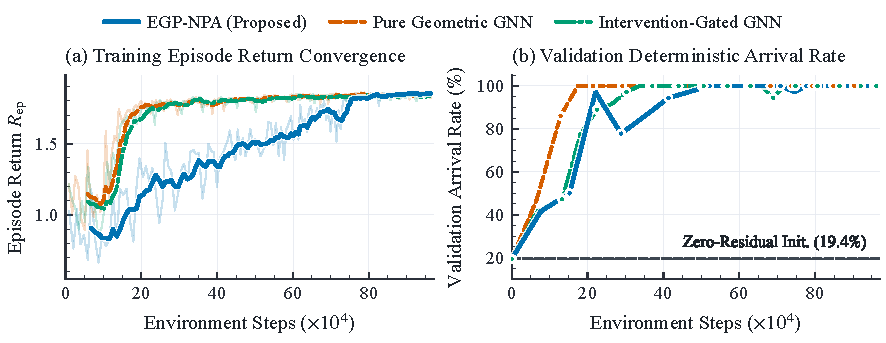
\includegraphics[width=\textwidth]{figures_en/fig2_training_curves.pdf}
 \caption{MAPPO training evolution over $9.6\times 10^5$ environment steps. (a) Episode return $R_{\mathrm{ep}}$ convergence (faint lines: raw episode returns; bold lines: moving average); (b) deterministic arrival rate on the $N=8$ validation benchmark ($36$ swap and permutation instances).}
 \label{fig:train-curves}
\end{figure*}

In \eqref{eq:nominal-law}, the tangential and radial residual terms scale with $\be_{i,k}$ and vanish as $\be_{i,k}\to\boldsymbol 0$, whereas the pairwise repulsive bias $\boldsymbol b_{i,k}^\psi=\frac{A_\psi U}{\max(|\mathcal N_{i,k}|,1)}\sum_{j\in\mathcal N_{i,k}}\psi_{ij,k}^\theta(\bp_{i,k}-\bp_{j,k})/d_{ij,k}$ is a zero-order term of unit direction vectors. On a tightly packed goal lattice with spacing $1.001\ \mathrm m$ ($1\ \mathrm{mm}$ above $\ds=1.000\ \mathrm m$), near-active contact constraints maintain $\norm{\boldsymbol\mu_{i,k-1}}_2>0$ and $\gamma_{i,k}^{\mathrm{gate}}\approx 1$, causing $\boldsymbol b_{i,k}^\psi$ to balance $-\be_{i,k}$ at $\norm{\be_{i,k}}_2\in[0.015,0.05]\ \mathrm m$ (terminal steady-state hovering).

To keep residuals active whenever any one-hop neighbor has not yet reached its goal while enforcing unconditional first-order vanishing once the entire one-hop closed neighborhood enters the goal ball, we define the \emph{One-Hop Closed-Neighborhood Completion Envelope}:
\begin{equation}
\begin{split}
 \rho_{i,k}(\bp_k)&=\tanh\!\left(\frac{\max_{j\in\mathcal N_{i,k}^+}\norm{\bp_{j,k}-\bg_j}_2}{\varepsilon_g}\right),\\
 \gamma_{i,k}^{\mathrm{eff}} &= \gamma_{i,k}^{\mathrm{gate}}\cdot\rho_{i,k}(\bp_k),
\end{split}\label{eq:envelope-def}
\end{equation}
with envelope scale $\varepsilon_g=0.05\ \mathrm m$ ($5\times$ the arrival tolerance $0.01\ \mathrm m$).

\begin{proposition}[First-Order Residual Vanishing and Goal Equilibrium Recovery]\label{prop:envelope}
Under the completion envelope \eqref{eq:envelope-def} in \eqref{eq:nominal-law}:
\begin{enumerate}
 \item \textbf{Residual preservation during cooperative transit:} Whenever there exists $j\in\mathcal N_{i,k}^+$ with $\norm{\be_{j,k}}_2\ge 3\varepsilon_g=0.15\ \mathrm m$, even if $\be_{i,k}=\boldsymbol 0$, we have $\rho_{i,k}(\bp_k)\ge\tanh(3)>0.995$.
 \item \textbf{First-order suppression near the goal and equilibrium restoration:} Let $e_{i,k}^{\max}:=\max_{j\in\mathcal N_{i,k}^+}\norm{\be_{j,k}}_2\le\norm{\be_k}_2$. Since $\tanh(z)\le z$ ($\forall z\ge 0$), $\gamma_{i,k}^{\mathrm{gate}}\in[0,1)$, and $|\omega_{i,k}^\theta|,|r_{i,k}^\theta|,|\psi_{ij,k}^\theta|\le 1$,
 \begin{equation}
 \begin{split}
  \norm{\gamma_{i,k}^{\mathrm{eff}}\br_{i,k}^\theta(\bp_k)}_2
  &\le \frac{e_{i,k}^{\max}}{\varepsilon_g}\Big[(A_{\mathrm{rot}}+A_{\mathrm{rad}})\norm{\be_{i,k}}_2+A_\psi U\Big]\\
  &=\mathcal O(\norm{\be_k}_2).
 \end{split}\label{eq:residual-bound}
 \end{equation}
 In particular, at $\bp_k=\bg$, $\rho_{i,k}(\bg)=0$ and $\bu_{i,k}^{\mathrm{nom}}(\bg;\theta)=\boldsymbol 0$ regardless of $\boldsymbol\mu_{i,k-1}$.
\end{enumerate}
\end{proposition}
\begin{proof}
Claim (1) follows from monotonicity of $\tanh(\cdot)$ since $\tanh(3)\approx 0.99505>0.995$. Claim (2) follows from $0\le\gamma_{i,k}^{\mathrm{eff}}\le\rho_{i,k}(\bp_k)\le e_{i,k}^{\max}/\varepsilon_g$ and the triangle inequality $\norm{\br_{i,k}^\theta(\bp_k)}_2\le(A_{\mathrm{rot}}+A_{\mathrm{rad}})\norm{\be_{i,k}}_2+A_\psi U$. Setting $\be_k=\boldsymbol 0$ yields $\bu_{i,k}^{\mathrm{nom}}(\bg;\theta)=\boldsymbol 0$.
\end{proof}

\subsection{Small-Scale Short-Horizon MAPPO Training and Zero-Shot Cross-Scale Deployment}\label{subsec:mappo}
Because the $B$-round block QP filter $L$ involves nonsmooth active-set switches and local settlements, backpropagating long-horizon policy gradients through the QP solver suffers from gradient singularities at multi-contact corners. We adopt a Centralized Training with Decentralized Execution (CTDE) MAPPO protocol \cite{yu2022mappo} that combines small-scale short-horizon training ($N\in\{6,\dots,10\},B=2$, validation selection on $N=8$) with large-scale multi-round zero-shot deployment ($N\in\{12,20,25\},B=8$), as summarized in Table~\ref{tab:algo1}. Training tasks are sampled on dense triangular lattices (spacing $1.001\sim 1.12\ \mathrm m$, $\lr/\lambda_2(\bp_0)\in[0.55,0.90]$, $1\sim 3$ pair swaps, 3-cycle rotations, and full permutations with random global rotation). The shared team reward at step $k$ is:
\begin{equation}
\begin{split}
 R_k &= r_{\mathrm{prog}}\frac{\sum_{i=1}^N\big(\norm{\be_{i,k}}_2-\norm{\be_{i,k+1}}_2\big)}{D_0} - r_{\mathrm{time}}\\
 &\quad + r_{\mathrm{succ}}\mathbb I\Big(\max_{i\in\mathcal V}\norm{\be_{i,k+1}}_2\le\varepsilon_{\mathrm{succ}}\Big)\\
 &\quad - \frac{r_{\mathrm{stall}}}{N}\sum_{i=1}^N\tanh\!\Big(\frac{\norm{\be_{i,k}}_2}{\varepsilon_p}\Big)\exp\!\Big(-\frac{\norm{\bu_{i,k}}_2^2}{\varepsilon_u^2}\Big)\\
 &\quad\qquad\qquad\times\ln\!\big(1+\norm{\boldsymbol\mu_{i,k}}_2^2\big),
\end{split}\label{eq:reward}
\end{equation}
where $D_0=\sum_{i=1}^N\norm{\be_{i,0}}_2$, $r_{\mathrm{prog}}=1.0$, $r_{\mathrm{time}}=10^{-3}$, $\varepsilon_{\mathrm{succ}}=0.01\ \mathrm m,r_{\mathrm{succ}}=1.0$, and the fourth term penalizes dual-blocked stagnation ($r_{\mathrm{stall}}=0.02,\varepsilon_p=0.10\ \mathrm m,\varepsilon_u=0.05\ \mathrm{m/s}$). Policy parameters $\theta$ are updated via GAE ($\gamma=0.995,\lambda_{\mathrm{GAE}}=0.95$) and clipped PPO ($\epsilon_{\mathrm{clip}}=0.20$, target KL $0.03$).

\begin{table}[htbp]
 \centering\footnotesize
 \caption{EGP-NPA Training and Zero-Shot Distributed Execution (Algorithm~1)}\label{tab:algo1}
 \renewcommand{\arraystretch}{1.10}
 \begin{tabularx}{\columnwidth}{@{}X@{}}
 \toprule
 \textbf{Phase A: Small-Scale Short-Horizon CTDE Training ($N\in\{6,\dots,10\},\ B_{\mathrm{train}}=2$)}\\
 \midrule
 1. Initialize 2-layer equivariant GNN actor $\theta$ and centralized GNN critic $\phi$;\\
 2. \textbf{for} iteration $m=1,2,\dots,M_{\max}$ \textbf{do}\\
 3. \hspace{0.8em}Sample dense triangular-lattice swap/permutation tasks ($N\in\{6,\dots,10\}$, random rotation), set $\boldsymbol\varpi_{-1}=\boldsymbol 0$;\\
 4. \hspace{0.8em}\textbf{for} step $k=0,1,\dots,K_{\max}-1$ \textbf{do}\\
 5. \hspace{1.6em}Construct invariant features $(\boldsymbol x_{i,k},\boldsymbol e_{ij,k}^{\mathrm{feat}})$ and sample noisy nominal velocity $\bu_{i,k}^{\mathrm{nom}}$ via \eqref{eq:gnn-layer}--\eqref{eq:nominal-law};\\
 6. \hspace{1.6em}Solve single-robot refit QP \eqref{eq:refit-one} (recording shadow prices $\boldsymbol\mu_{i,k}$) and apply one-hop local settlement if needed;\\
 7. \hspace{1.6em}Run $B_{\mathrm{train}}=2$ closed-neighborhood block NPA rounds \eqref{eq:block-qp}--\eqref{eq:convex-commit} and ZOH certificate (Theorem~\ref{thm:zoh-safe});\\
 8. \hspace{1.6em}Compute team reward $R_k$ via \eqref{eq:reward} and store transition in rollout buffer;\\
 9. \hspace{0.8em}\textbf{end for}\\
 10. \hspace{0.4em}Compute GAE advantages, update $(\theta,\phi)$ via clipped PPO, and save best checkpoint $\theta^\star$ on $N=8$ validation set.\\
 11. \textbf{end for}\\
 \midrule
 \textbf{Phase B: Zero-Shot Cross-Scale Decentralized Execution (Arbitrary $N$, $\theta=\theta^\star,\ B_{\mathrm{eval}}=8$)}\\
 \midrule
 12. At each step $t_k$, each robot $i\in\mathcal V$ evaluates completion envelope $\rho_{i,k}(\bp_k)=\tanh(\max_{j\in\mathcal N_{i,k}^+}\norm{\be_{j,k}}_2/\varepsilon_g)$;\\
 13. Compute deterministic GNN actions $(\omega_{i,k}^{\theta^\star},r_{i,k}^{\theta^\star},\psi_{ij,k}^{\theta^\star})$ and synthesize $\bu_{i,k}^{\mathrm{nom}}(\bp_k;\theta^\star)$ via \eqref{eq:nominal-law};\\
 14. Execute single-robot refit \eqref{eq:refit-one}, one-hop settlement, and $B_{\mathrm{eval}}=8$ block NPA rounds \eqref{eq:block-qp}--\eqref{eq:convex-commit} to apply $\bu_{i,k}$.\\
 \bottomrule
 \end{tabularx}
\end{table}

\section{Closed-Loop Numerical Validation, Mechanism Decomposition, and Virtual-Physical Verification}\label{sec:experiments}

\subsection{Experimental Setup, Baselines, and Evaluation Metrics}
We evaluate EGP-NPA across training-scale ($N=8$) and zero-shot cross-scale transfer ($N\in\{12,20,25\}$) dense triangular-lattice swap and random full-permutation benchmarks. All experiments share identical physical and safety parameters: $\ds=1.000\ \mathrm m$, $U=0.50\ \mathrm{m/s}$, $B_{\mathrm{ws}}=4.0\ \mathrm m$, $R_c=10.0\ \mathrm m$, $R_{\mathrm{sense}}=2.50\ \mathrm m$, $\alpha_c=\alpha_s=\alpha_x=2.0\ \mathrm s^{-1}$, $\Delta t=0.05\ \mathrm s$, and horizon $T_{\max}=60.0\ \mathrm s$. Initial configurations are tightly packed triangular lattices with spacing $1.001\ \mathrm m$ ($1.0\ \mathrm{mm}$ initial clearance). Fig.~\ref{fig:train-curves} shows the MAPPO training return and deterministic validation arrival rate ($N=8$, $36$ validation instances) over $9.6\times 10^5$ environment steps: the zero-residual initialization (myopic proportional attraction) achieves only $19.4\%$ arrival, whereas EGP-NPA converges to $100\%$ validation arrival.

\begin{table*}[t]
 \centering\footnotesize
 \caption{Closed-Loop Comparison on the Training-Scale Benchmark ($N=8$, $32$ Instances Each at $f=0.60$ and $f=0.90$) Against Three Safe RL Methods and Two Classical Baselines}\label{tab:e1}
 \begin{tabularx}{\textwidth}{@{}Xcccccc@{}}
 \toprule
 Control Method & $f=0.60$ Arrival & Median Time & $f=0.90$ Arrival & Median Time & Step Cuts & Audit Viol.\\
 \midrule
 \textbf{EGP-NPA (Proposed)} & $\mathbf{32/32\ (100\%)}$ & $\mathbf{7.32\ \mathrm s}$ & $\mathbf{32/32\ (100\%)}$ & $\mathbf{7.12\ \mathrm s}$ & $\mathbf{0}$ & $\mathbf{0}$\\
 Shield-Consistent Safe MARL (\texttt{Proj-MAPPO + NPA} \cite{wabersich2021,liu2026saferl}, $B=8$) & $32/32\ (100\%)$ & $9.53\ \mathrm s$ & $32/32\ (100\%)$ & $10.73\ \mathrm s$ & $0$ & $0$\\
 Decentralized Static-CBF GNN (\texttt{Static-CBF GNN} \cite{zhang2025gcbf,zhang2025dgppo}, $B=0$) & $5/32\ (15.6\%)$ & $13.30\ \mathrm s$ & $6/32\ (18.8\%)$ & $13.88\ \mathrm s$ & $431\,725$ & $0$\\
 Primal-Dual Safe MARL (\texttt{MAPPO-Lagrangian} \cite{gu2023safe}, Unshielded) & $0/32^\ddagger\ (0\%)$ & $4.15\ \mathrm s^\ddagger$ & $0/32^\ddagger\ (0\%)$ & $4.15\ \mathrm s^\ddagger$ & --- & $7\,029$\\
 Circulation Heuristic \cite{goncalves2023circulation} + Dynamic NPA ($B=8$) & $21/32\ (65.6\%)$ & $32.50\ \mathrm s$ & $18/32\ (56.3\%)$ & $30.50\ \mathrm s$ & $0$ & $0$\\
 Myopic CBF Filter \cite{ames2017cbf,reis2021} + Dynamic NPA ($B=8$) & $17/32\ (53.1\%)$ & $36.35\ \mathrm s$ & $16/32\ (50.0\%)$ & $31.80\ \mathrm s$ & $0$ & $0$\\
 Circulation Heuristic + Static Equal Split \cite{ames2017cbf,zhang2025gcbf} ($B=0$) & $2/32\ (6.3\%)$ & $25.10\ \mathrm s$ & --- & --- & $72\,156$ & $0$\\
 \bottomrule
 \end{tabularx}
 \vspace{1.5pt}
 \par\raggedright\scriptsize Note: $^\ddagger$\texttt{MAPPO-Lagrangian} reaches the goal vicinity in $64/64$ runs (median $4.15\ \mathrm s$) but violates collision safety on all $64$ runs ($7\,029$ violated ZOH segments, median $\min d_{ij}=0.263\ \mathrm m<\ds=1.000\ \mathrm m$), yielding $0/32$ safe arrivals.
\end{table*}

The primary benchmark comprises $96$ independent instances:
\begin{enumerate}
 \item \textbf{Training-scale benchmark ($N=8$, $64$ instances):} $20$ local pair-swap instances ($1\sim 3$ adjacent pairs swap goals while remaining nodes stay at their goals) and $12$ random full-permutation instances, evaluated under both nominal connectivity threshold $f=\lr/\lambda_2(\bp_0)=0.60$ ($32$ instances) and tight connectivity threshold $f=0.90$ ($32$ instances).
 \item \textbf{Zero-shot cross-scale transfer benchmark ($N\in\{12,20,25\}$, $32$ instances):} $N=12$ ($8$ local swaps + $4$ full permutations), $N=20$ ($8$ local swaps + $4$ full permutations), and $N=25$ ($8$ local swaps) at $f=0.60$, directly deploying the frozen small-scale checkpoint $\theta^\star$ without retraining.
\end{enumerate}

We compare EGP-NPA against \textbf{three representative Safe MARL baselines} and \textbf{three classical analytical/heuristic CBF baselines}:
\begin{enumerate}
 \item \textbf{Shield-Consistent / Action-Projected Safe MARL (\texttt{Proj-MAPPO + NPA} \cite{wabersich2021,liu2026saferl}):} Represents recent predictive/adaptive safety-filter RL frameworks that penalize filter intervention during training. It shares the identical 2-layer equivariant GNN, completion envelope $\rho_{i,k}$, and $B=8$ closed-neighborhood NPA shield, but adds the shield-projection consistency loss $\mathcal L_{\mathrm{proj}}(\theta)=\lambda_{\mathrm{proj}}\frac1N\sum_{i=1}^N\norm{\Pi_{\mathcal U_i}(\bu_{i,k}^{\mathrm{nom}}(\theta))-\operatorname{sg}(\bu_{i,k})}_2^2$ ($\lambda_{\mathrm{proj}}=1.0$ calibrated by gradient norm ratio) to align nominal actions with filtered safe velocities;
 \item \textbf{Decentralized Static-CBF Shielded GNN (\texttt{Static-CBF GNN}, GCBF+/DGPPO paradigm \cite{zhang2025gcbf,zhang2025dgppo}):} Represents neural graph CBF / decentralized static-split safe MARL methods, combining the equivariant GNN policy and completion envelope $\rho_{i,k}$ with decentralized single-agent static-split CBF-QP filtering ($B=0$, $s_{ia,k}\equiv 0$, without dynamic quota transfer $t_e$);
 \item \textbf{Primal-Dual Constrained Safe MARL (\texttt{MAPPO-Lagrangian} \cite{gu2023safe}):} Represents model-free Constrained Markov Decision Process (CMDP) safe MARL without a hard coupled QP shield, training the identical 2-layer equivariant GNN actor, task critic, and cost critic with an adaptive dual-ascent Lagrangian multiplier $\lambda_{\mathrm{lag}}\ge 0$ penalizing collision and connectivity violations;
 \item \textbf{Classical Analytical and Heuristic CBF Baselines:} Tangential Circulation Heuristic of Gon\c{c}alves et al. \cite{goncalves2023circulation} ($\omega_i\equiv 1,r_i\equiv 0,\psi_{ij}\equiv 0$ with $B=8$), Myopic Proportional Attraction CBF filtering of Ames et al. \cite{ames2017cbf,reis2021} ($\bu_i^{\mathrm{nom}}=-\be_i$ with $B=8$), and Circulation Heuristic with static quota splitting ($B=0$).
\end{enumerate}
Safe arrival requires $\max_{i\in\mathcal V}\norm{\bp_i(t)-\bg_i}_2\le 0.01\ \mathrm m$ maintained continuously for $1.0\ \mathrm s$ with $0$ rational safety audit violations across all ZOH segments (Theorem~\ref{thm:zoh-safe}). Statistical significance is evaluated via two-sided McNemar exact binomial tests on discordant pairs and median paired arrival-time differences $\Delta t$ on common arrivals.

\subsection{Closed-Loop State Evolution on Dense Interior Swap and Full Permutation}
Figs.~\ref{fig:swap-traj} and \ref{fig:time-evol} compare the spatial trajectories, communication topologies, and closed-loop time responses on a representative $N=20$ interior pair-swap task ($2$ interior robots swap positions while $18$ outer robots start at their goals).

\begin{figure*}[t]
 \centering
 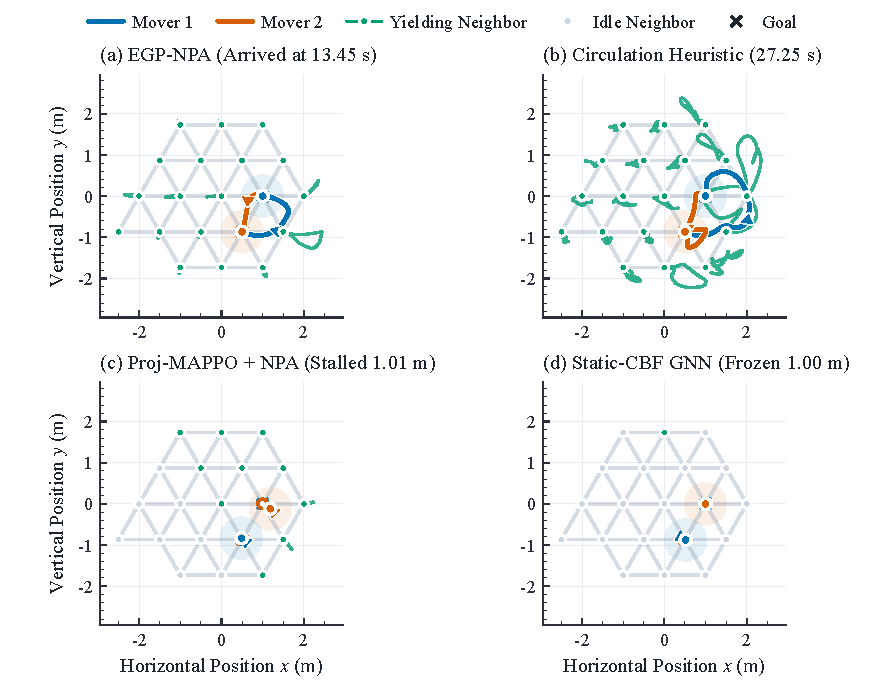
\includegraphics[width=\textwidth]{figures_en/fig3_swap_trajectory.pdf}
 \caption{Spatial trajectories and communication topologies on the $N=20$ dense triangular-lattice interior pair-swap task. (a) EGP-NPA drives the swapping pair along smooth tangential bypasses while unfreezing outer stationary neighbors (bluish-green loops) via dynamic quota transfer, arriving at $13.45\ \mathrm s$; (b) Circulation Heuristic \cite{goncalves2023circulation} triggers large-scale rotational conflicts among outer neighbors ($27.25\ \mathrm s$); (c) Shield-Consistent Safe MARL (\texttt{Proj-MAPPO + NPA} \cite{wabersich2021,liu2026saferl}) stalls in a livelock at $1.01\ \mathrm m$ because penalizing normal filter modification weakens the yielding drive $\delta_n>0$; (d) Decentralized Static-CBF GNN (\texttt{Static-CBF GNN} \cite{zhang2025gcbf,zhang2025dgppo}, $B=0$) freezes at $1.00\ \mathrm m$ due to static quota splitting.}
 \label{fig:swap-traj}
\end{figure*}

\begin{table*}[t]
 \centering\footnotesize
 \caption{Zero-Shot Cross-Scale Transfer Benchmark ($N\in\{12,20,25\}$, $32$ Instances Total) Against Three Safe RL Methods and Two Classical Baselines}\label{tab:e2}
 \begin{tabularx}{\textwidth}{@{}Xccccccr@{}}
 \toprule
 Control Method & $N=12$ ($12$) & $N=20$ ($12$) & $N=25$ ($8$) & Total Arrival ($32$) & Discordant ($p$-val) & Median $\Delta t$ & Step Cuts\\
 \midrule
 \textbf{EGP-NPA (Proposed)} & $\mathbf{12/12\ (6.52\ \mathrm s)}$ & $\mathbf{12/12\ (10.55\ \mathrm s)}$ & $\mathbf{8/8\ (10.43\ \mathrm s)}$ & $\mathbf{32/32\ (100\%)}$ & Baseline & Baseline & $\mathbf{0}$\\
 Proj-MAPPO + NPA \cite{wabersich2021,liu2026saferl} ($B=8$) & $9/12\ (17.25\ \mathrm s)$ & $5/12\ (17.70\ \mathrm s)$ & $3/8\ (12.30\ \mathrm s)$ & $17/32\ (53.1\%)$ & $15:0\ (6.1\times 10^{-5})$ & $-3.85\ \mathrm s$ & $0$\\
 Static-CBF GNN \cite{zhang2025gcbf,zhang2025dgppo} ($B=0$) & $0/12\ (\text{---})$ & $0/12\ (\text{---})$ & $1/8\ (19.85\ \mathrm s)$ & $1/32\ (3.1\%)$ & $31:0\ (9.3\times 10^{-10})$ & $-12.95\ \mathrm s$ & $447\,022$\\
 MAPPO-Lagrangian \cite{gu2023safe} (Unshielded) & $0/12^\ddagger\ (4.05\ \mathrm s)$ & $0/12^\ddagger\ (3.95\ \mathrm s)$ & $0/8^\ddagger\ (3.92\ \mathrm s)$ & $0/32^\ddagger\ (0\%)$ & $32:0\ (4.7\times 10^{-10})$ & --- & $3\,900^\ddagger$\\
 Circulation Heuristic \cite{goncalves2023circulation} & $7/12\ (14.40\ \mathrm s)$ & $4/12\ (24.53\ \mathrm s)$ & $2/8\ (38.22\ \mathrm s)$ & $13/32\ (40.6\%)$ & $19:0\ (3.8\times 10^{-6})$ & $-12.35\ \mathrm s$ & $14\,198$\\
 Myopic CBF Filter \cite{ames2017cbf,reis2021} & $4/12\ (34.30\ \mathrm s)$ & $1/12\ (55.50\ \mathrm s)$ & $0/8\ (\text{---})$ & $5/32\ (15.6\%)$ & $27:0\ (1.5\times 10^{-8})$ & $-26.70\ \mathrm s$ & $0$\\
 \bottomrule
 \end{tabularx}
 \vspace{1.5pt}
 \par\raggedright\scriptsize Note: All five shielded methods incur $0$ rational audit violations; $^\ddagger$\texttt{MAPPO-Lagrangian} violates collision safety on all $32$ cross-scale runs ($3\,900$ violated ZOH segments recorded in the last column, median $\min d_{ij}=0.263\ \mathrm m<\ds$), yielding $0/32$ safe arrivals.
\end{table*}

\begin{figure*}[t]
 \centering
 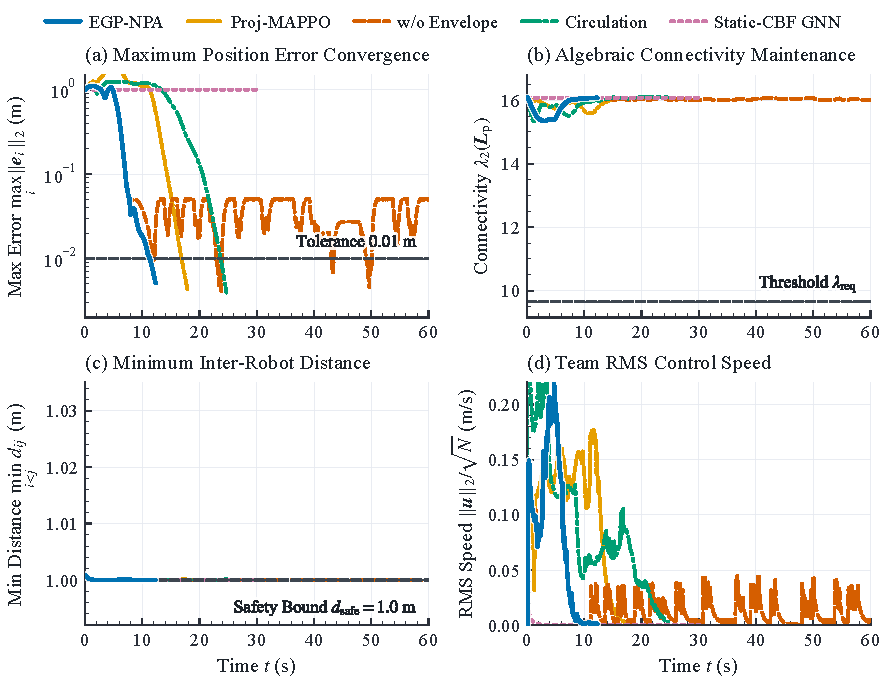
\includegraphics[width=\textwidth]{figures_en/fig4_time_evolution.pdf}
 \caption{Closed-loop time responses on the $N=20$ interior swap task. (a) Maximum position error $\max_i\norm{\be_i(t)}_2$ (log scale); (b) algebraic connectivity $\lambda_2(\bL(t))$ vs. $\lr=9.69$; (c) minimum inter-robot distance $\min_{i<j}d_{ij}(t)$ vs. $\ds=1.0\ \mathrm m$; (d) team RMS control speed $\norm{\bu(t)}_2/\sqrt{N}$.}
 \label{fig:time-evol}
\end{figure*}

Three physical mechanisms are evident from Figs.~\ref{fig:swap-traj} and \ref{fig:time-evol}:
\begin{enumerate}
 \item \textbf{Chiral lateral bypass and stationary neighbor yielding--return loop:} Under Decentralized Static-CBF GNN (\texttt{Static-CBF GNN}, $B=0$, Fig.~\ref{fig:swap-traj}(d)), outer stationary target-holding neighbors refuse to yield collision quotas, truncating the swapping pair's lateral velocity and driving RMS speed to zero (purple dotted curve in Fig.~\ref{fig:time-evol}(d)). Under Shield-Consistent Safe MARL (\texttt{Proj-MAPPO + NPA}, Fig.~\ref{fig:swap-traj}(c)), penalizing normal filter intervention weakens the normal intrusion $\delta_n>0$, trapping the swapping pair in a local livelock at $1.01\ \mathrm m$ (or arriving slowly at $16.90\ \mathrm s$ in Fig.~\ref{fig:time-evol}(a)). Under EGP-NPA (Fig.~\ref{fig:swap-traj}(a)), the equivariant GNN generates chiral tangential thrust for the swapping pair, and closed-neighborhood dynamic quota transfer converts this lateral push into compact outward yielding loops (bluish-green trajectories) of adjacent stationary neighbors, which smoothly return to their goals once the swapping pair passes.
 \item \textbf{Elimination of terminal steady-state hovering by the completion envelope:} In Fig.~\ref{fig:time-evol}(a) and (d), the ablation without the completion envelope (orange dashed curve) resolves the initial deadlock within $8\ \mathrm s$ but remains trapped in a limit cycle at $\max_i\norm{\be_i}_2\in[0.015,0.05]\ \mathrm m$ with persistent RMS speed $0.01\sim 0.04\ \mathrm{m/s}$ due to nonvanishing zero-order repulsive bias $\boldsymbol b_{i,k}^\psi$. With the one-hop completion envelope $\rho_{i,k}$ \eqref{eq:envelope-def}, residuals vanish to first order inside $\varepsilon_g=0.05\ \mathrm m$ (Proposition~\ref{prop:envelope}), driving the error cleanly below $0.01\ \mathrm m$ and bringing control speed to zero.
 \item \textbf{Strict continuous-time safety invariance:} Throughout the maneuver (Fig.~\ref{fig:time-evol}(b)--(c)), $\lambda_2(\bL(t))\ge 15.3>\lr=9.69$ and $\min_{i<j}d_{ij}(t)\ge\ds=1.000\ \mathrm m$ with zero violations.
\end{enumerate}

\subsection{Comparison With External Baselines on Training and Cross-Scale Benchmarks}
Tables~\ref{tab:e1} and \ref{tab:e2} summarize the statistical results across the $64$ training-scale instances ($N=8$) and $32$ zero-shot cross-scale instances ($N\in\{12,20,25\}$), establishing four key findings:
\begin{enumerate}
 \item \textbf{Unshielded constrained MARL (\texttt{MAPPO-Lagrangian} \cite{gu2023safe}) fails to maintain hard safety on millimeter-clearance lattices:} Despite dual ascent raising the Lagrangian multiplier to $\lambda_{\mathrm{lag}}=2.45$, soft penalty gradients cannot prevent inter-robot penetration during counter-crossing on tightly packed lattices ($1.0\ \mathrm{mm}$ initial clearance), incurring $10\,929$ violated ZOH segments across all $96$ runs ($0\%$ safe arrival rate) and confirming Proposition~\ref{prop:safety}.
 \item \textbf{Decentralized static-CBF shielded GNN (\texttt{Static-CBF GNN} \cite{zhang2025gcbf,zhang2025dgppo}, $B=0$) freezes under multi-layer stationary wrapping:} Sharing the exact same GNN policy weights and completion envelope as EGP-NPA but using static equal responsibility splitting ($B=0$), \texttt{Static-CBF GNN} achieves only $17.2\%$ ($11/64$) arrival on $N=8$ ($431\,725$ step cuts) and collapses to $3.1\%$ ($1/32$, discordant pairs $31:0,p=9.3\times 10^{-10}$) on $N\in\{12,20,25\}$, directly verifying Proposition~\ref{prop:unfreeze} Claim~1.
 \item \textbf{Shield-consistent safe MARL (\texttt{Proj-MAPPO + NPA} \cite{wabersich2021,liu2026saferl}) degrades cross-scale deadlock resolution:} While achieving $64/64$ arrival on $N=8$ (albeit $2.88\ \mathrm s$ slower in median time), its zero-shot cross-scale arrival rate drops to $53.1\%$ ($17/32$, discordant pairs $15:0,p=6.1\times 10^{-5}$, $-3.85\ \mathrm s$ slower) on $N\in\{12,20,25\}$ because penalizing filter intervention suppresses the normal intrusion $\delta_n>0$ required by Proposition~\ref{prop:unfreeze} Claim~2 to push open multi-layer stationary neighbors.
 \item \textbf{Superiority over classical analytical/heuristic baselines:} As $N$ scales to $25$, Myopic CBF filtering and Circulation Heuristic drop to $15.6\%$ ($27:0,p=1.5\times 10^{-8}$) and $40.6\%$ ($19:0,p=3.8\times 10^{-6}$), whereas EGP-NPA achieves $96/96$ ($100\%$) safe arrival with $0$ step cuts and $0$ audit violations.
\end{enumerate}

\subsection{Internal Module Ablation, Velocity Decomposition, and Holdout Factorial Analysis}\label{subsec:ablation}
Table~\ref{tab:decomp} reports: (A) cross-scale ablations removing the completion envelope ($\rho_{i,k}\equiv 1$) and comparing training checkpoints; (B) deadlock-breaking velocity decomposition on $N=20$ ($t\in[0.05,1.00]\ \mathrm s$) under identical EGP-NPA nominal inputs comparing dynamic allocation ($B=8$) vs. static splitting ($B=0$); and (C) controlled single-variable execution-time interventions holding the trained weights $\theta^\star$ strictly fixed ($16$ cross-scale instances; Fig.~\ref{fig:perm-gate}(b)).

\begin{figure*}[t]
 \centering
 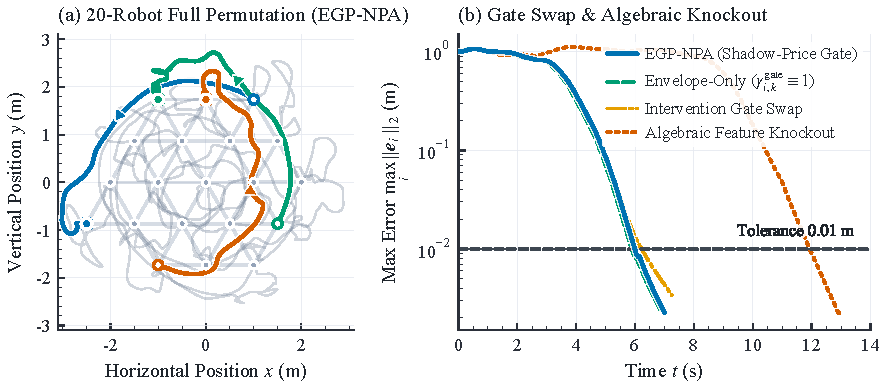
\includegraphics[width=\textwidth]{figures_en/fig5_perm_and_gate.pdf}
 \caption{Twenty-robot full-permutation trajectories and fixed-weight gate replacement and feature knockout responses. (a) Spatial trajectories of EGP-NPA on $N=20$ random full permutation (slate lines: background fleet; colored bold curves: three large-span crossing robots); (b) maximum error convergence under fixed policy weights $\theta^\star$ comparing shadow-price gate $\gamma^{\mathrm{gate},\mu}$, envelope-only gate $\gamma^{\mathrm{gate}}\equiv 1$, intervention gate swap $\gamma^{\mathrm{gate,int}}$, and algebraic feature knockout.}
 \label{fig:perm-gate}
\end{figure*}

\begin{table*}[t]
 \centering\footnotesize
 \caption{Internal Module Cross-Scale Ablation (Part A, $32$ Instances), Deadlock-Breaking Velocity Decomposition (Part B, $t\in[0.05,1.00]\ \mathrm s$), and Fixed-Weight ($\theta^\star$) Single-Variable Execution Interventions (Part C, $16$ Instances)}\label{tab:decomp}
 \begin{tabularx}{\textwidth}{@{}Xccccr@{}}
 \toprule
 A. Cross-Scale Module Ablation ($32$ Instances) & $N=12$ ($12$) & $N=20$ ($12$) & $N=25$ ($8$) & Total Arrival ($32$) & Discordant ($p$-val) / $\Delta t$\\
 \midrule
 \textbf{EGP-NPA (Full Architecture)} & $12/12\ (6.52\ \mathrm s)$ & $12/12\ (10.55\ \mathrm s)$ & $8/8\ (10.43\ \mathrm s)$ & $\mathbf{32/32\ (100\%)}$ & Baseline\\
 w/o Completion Envelope (fixed $\theta^\star$, $\rho_{i,k}\equiv 1$) & $12/12\ (9.78\ \mathrm s)$ & $5/12\ (36.75\ \mathrm s)$ & $8/8\ (14.10\ \mathrm s)$ & $25/32\ (78.1\%)$ & $7:0\ (0.0156)$ / $-2.40\ \mathrm s$\\
 Pure Geometric GNN (trained w/o algebraic features) & $12/12\ (7.57\ \mathrm s)$ & $7/12\ (21.90\ \mathrm s)$ & $3/8\ (19.65\ \mathrm s)$ & $22/32\ (68.8\%)$ & $10:0\ (0.0020)$ / $-0.45\ \mathrm s$\\
 Intervention-Gated GNN ($\gamma_{i,k}^{\mathrm{gate,int}}$ checkpoint) & $10/12\ (11.20\ \mathrm s)$ & $4/12\ (30.08\ \mathrm s)$ & $1/8\ (6.80\ \mathrm s)$ & $15/32\ (46.9\%)$ & $17:0\ (1.5\times 10^{-5})$ / $-0.50\ \mathrm s$\\
 \midrule
 \multicolumn{4}{@{}l}{B. Velocity Decomposition Under Identical EGP-NPA Input ($N=20$ Swap)} & Dynamic ($B=8$) & Static ($B=0$)\\
 \midrule
 \multicolumn{4}{@{}l}{Swapping robots' mean tangential (lateral) nominal speed $|\hat{\be}_i^{\top}\bJ^{\top}\bu_i^{\mathrm{nom}}|$} & $0.8887\ \mathrm{m/s}$ & $0.8887\ \mathrm{m/s}$\\
 \multicolumn{4}{@{}l}{Swapping robots' mean tangential (lateral) executed speed $|\hat{\be}_i^{\top}\bJ^{\top}\bu_i|$} & $\mathbf{0.2003\ \mathrm{m/s}}$ & $0.0004\ \mathrm{m/s}$\\
 \multicolumn{4}{@{}l}{Outer 1-hop stationary neighbors' mean outward nominal residual speed} & $-0.0105\ \mathrm{m/s}$ & $-0.0105\ \mathrm{m/s}$\\
 \multicolumn{4}{@{}l}{Outer 1-hop stationary neighbors' mean outward executed yielding speed} & $\mathbf{+0.0915\ \mathrm{m/s}}$ & $+0.0013\ \mathrm{m/s}$\\
 \midrule
 C. Fixed-Weight ($\theta^\star$) Execution-Time Interventions ($16$ Instances) & $N=12$ ($6$) & $N=20$ ($6$) & $N=25$ ($4$) & Arrival ($16$) & Paired $\Delta t$ / Cuts\\
 \midrule
 Native shadow-price gate $\gamma_{i,k}^{\mathrm{gate},\mu}$ & $6/6\ (6.52\ \mathrm s)$ & $6/6\ (11.48\ \mathrm s)$ & $4/4\ (9.98\ \mathrm s)$ & $16/16\ (100\%)$ & Baseline / $0$\\
 Stateless envelope-only gate ($\gamma_{i,k}^{\mathrm{gate}}\equiv 1$, retaining only $\rho_{i,k}$) & $6/6\ (6.40\ \mathrm s)$ & $6/6\ (10.03\ \mathrm s)$ & $4/4\ (9.73\ \mathrm s)$ & $16/16\ (100\%)$ & $-0.10\ \mathrm s$ / $0$\\
 Filter-intervention gate replacement ($\gamma_{i,k}^{\mathrm{gate,int}}$ at execution) & $6/6\ (6.82\ \mathrm s)$ & $6/6\ (9.35\ \mathrm s)$ & $4/4\ (10.43\ \mathrm s)$ & $16/16\ (100\%)$ & $+0.33\ \mathrm s$ / $0$\\
 Post-negotiation multiplier extraction with cross-step EMA & $6/6\ (7.03\ \mathrm s)$ & $6/6\ (12.48\ \mathrm s)$ & $4/4\ (9.73\ \mathrm s)$ & $16/16\ (100\%)$ & $+0.03\ \mathrm s$ / $0$\\
 In-distribution knockout of collision shadow prices ($4$ cols zeroed) & $6/6\ (7.63\ \mathrm s)$ & $6/6\ (13.38\ \mathrm s)$ & $4/4\ (10.50\ \mathrm s)$ & $16/16\ (100\%)$ & $\mathbf{+1.18\ \mathrm s}\ (p=0.0042)$ / $0$\\
 In-distribution knockout of collision edge ledgers ($\varpi_{ij,1}=0$) & $6/6\ (6.40\ \mathrm s)$ & $6/6\ (10.03\ \mathrm s)$ & $4/4\ (9.80\ \mathrm s)$ & $16/16\ (100\%)$ & $0.00\ \mathrm s\ (p=1.0)$ / $0$\\
 Zeroing all $12$ algebraic features (including constant reserve col.) & $6/6\ (9.85\ \mathrm s)$ & $5/6\ (9.80\ \mathrm s)$ & $4/4\ (13.03\ \mathrm s)$ & $15/16\ (93.8\%)$ & $+1.30\ \mathrm s\ (p=0.0074)$ / $2\,193$\\
 \bottomrule
 \end{tabularx}
\end{table*}

Table~\ref{tab:decomp} confirms three causal mechanisms:
\begin{enumerate}
 \item \textbf{Completion envelope necessity (Part A):} Removing $\rho_{i,k}$ while holding $\theta^\star$ fixed induces $7$ terminal hovering failures on $N=20$ ($7:0,p=0.0156$, $+2.40\ \mathrm s$ slower), directly verifying Proposition~\ref{prop:envelope}. Note that the pure-geometric and intervention-gated rows in Part~A reflect independently trained single-seed checkpoints (whose differences combine configuration effects with inter-seed training variance), whereas Parts~B and C isolate strict causal effects under fixed weights $\theta^\star$.
 \item \textbf{Division of labor between learned lateral intrusion and dynamic quota yielding (Part B):} During deadlock breaking, the GNN outputs a lateral nominal speed of $0.8887\ \mathrm{m/s}$ for the swapping pair (with $0.000$ action saturation across all runs), while stationary neighbors output virtually zero outward nominal residual ($-0.0105\ \mathrm{m/s}$). Under $B=8$ dynamic allocation, block QPs transfer collision quotas to drive stationary neighbors outward at $+0.0915\ \mathrm{m/s}$, allowing swapping nodes to advance laterally at $0.2003\ \mathrm{m/s}$; under static splitting ($B=0$), these speeds collapse to $+0.0013\ \mathrm{m/s}$ and $0.0004\ \mathrm{m/s}$, confirming Proposition~\ref{prop:unfreeze}.
 \item \textbf{Execution-time gate simplification and feature knockout (Part C):} Holding $\theta^\star$ fixed, setting $\gamma_{i,k}^{\mathrm{gate}}\equiv 1$ (retaining only $\rho_{i,k}$) achieves $16/16$ arrival with trajectories indistinguishable from $\gamma_{i,k}^{\mathrm{gate},\mu}$ (Fig.~\ref{fig:perm-gate}(b)). Across all $32$ cross-scale instances, zeroing only the $4$ collision shadow-price columns reduces arrival to $31/32$ and slows down $25$ of $31$ common arrivals (two-sided sign test $p=8.8\times 10^{-4}$; $+1.18\ \mathrm s$ on the $16$-instance subset), proving active utilization of refit shadow prices $\boldsymbol\mu_{i,k-1}$, whereas zeroing collision ledgers or replacing the $3$ Laplacian eigenvector columns with their median constant yields $32/32$ arrival with $0.00\ \mathrm s$ median difference.
\end{enumerate}

On $48$ additional independent holdout instances ($32$ at $N=8$ and $16$ at $N\in\{12,20,25\}$) plus $2$ exact mirror-symmetric head-on swap benchmarks, EGP-NPA again achieves $100\%$ arrival and $0$ violations. Controlled factorial tests show that: (1) enforcing $\mathrm{O}(2)$ reflection equivariance via odd--even feature symmetrization forces $\mathrm{mean}|\omega|=0.0000$ on symmetric head-on swaps (100\% deadlock) and drops holdout arrival from $48/48$ to $30/48$ ($62.5\%,p=7.6\times 10^{-6}$), confirming Proposition~\ref{prop:equivariance}; (2) adding a shield projection consistency loss $\norm{\Pi_{\mathcal U_i}(\bu_{i,k}^{\mathrm{nom}})-\operatorname{sg}(\bu_{i,k})}_2^2$ reduces filter intervention by $40\%\sim 70\%$ but slows common arrivals by $+2.00\ \mathrm s$ ($p=6.2\times 10^{-9}$) by suppressing normal intrusion $\delta_n>0$; and (3) replacing the global pooled critic with a local neighborhood critic delays convergence by $16\sim 24$ iterations since $2.50\ \mathrm m$ neighborhoods already cover $91.5\%$ of the team at $N\le 10$. Increasing evaluation rounds from $B=2$ to $B=8$ on $N=8$ reduces median arrival time from $8.07\ \mathrm s$ to $7.42\ \mathrm s$ ($32/32$ arrival for both), within $0.33\ \mathrm s$ of exact centralized per-step QP ($B\to\infty$) owing to cross-step ledger persistence.

\subsection{Zero-Shot Virtual-Physical Verification on Second-Order Chassis in MuJoCo}\label{subsec:mujoco}
Finally, we evaluate zero-shot transfer of the frozen single-integrator EGP-NPA policy $\theta^\star$ and completion envelope $\rho_{i,k}$ when integrated with an online division-free 3-channel distributed spectral estimator ($6$ consensus rounds per step) and deployed on second-order omnidirectional robots in \texttt{MuJoCo 3.6.0} ($200\ \mathrm{Hz}$ physics step $\delta t=5\ \mathrm{ms}$, robot mass $m=6.0\ \mathrm{kg}$, body radius $r_{\mathrm{body}}=0.45\ \mathrm m$, velocity-loop time constant $\tau_v=45\ \mathrm{ms}$, thrust limit $F_{\max}=22.0\ \mathrm N$, control period $\Delta t=0.05\ \mathrm s$, observation delay $10\ \mathrm{ms}$, packet delay $\tau_{\mathrm{comm}}\in[5,15]\ \mathrm{ms}$, packet drop rate $2\%$, and $B=4$ block NPA rounds).

\begin{table*}[t]
 \centering\footnotesize
 \caption{Full-Stack \texttt{MuJoCo} Second-Order Chassis Verification Combining EGP-NPA, Online Division-Free Spectral Estimation, and Closed-Neighborhood NPA Across Two Physical Compensation Regimes ($\ds=1.000\ \mathrm m$; $0$ Connectivity Violations in All $64$ Runs)}\label{tab:mujoco}
 \setlength{\tabcolsep}{4.5pt}
 \begin{tabularx}{\textwidth}{@{}lcXrrrrrr@{}}
 \toprule
 Regime & Scale & System Configuration & Arrival (Mean) & $\min_t d_{ij}$ (m) & Viol. Steps & $\min_t\lambda_2$ & $\hat{\lambda}_2$ RMSE & Final Err. (m)\\
 \midrule
 \textbf{Regime A} & $N=8$ & Myopic Attraction + Phys-NPA & $0/4$ (---) & $0.9817$ & $610.2$ & $6.963$ & $0.0273$ & $1.394$\\
 (Look-Ahead, & & EGP-NPA + Static Split ($B=0$) & $1/4$ ($10.12\ \mathrm s$) & $0.9798$ & $442.2$ & $6.847$ & $0.0318$ & $1.353$\\
 $S=1.018\ \mathrm m$) & & EGP-NPA + Ideal Single-Integrator NPA & $0/4$ (---) & $0.9792$ & $4\,231.0$ & $7.071$ & $0.0268$ & $1.653$\\
 & & \textbf{EGP-NPA + Online Est. + Phys-NPA (Full)} & $\mathbf{3/4}$ ($\mathbf{13.88\ \mathrm s}$) & $0.8990$ & $1\,683.5$ & $6.670$ & $0.0337$ & $\mathbf{0.629}$\\
 \cmidrule{2-9}
 & $N=12$ & Myopic Attraction + Phys-NPA & $0/4$ (---) & $0.9952$ & $1\,679.2$ & $10.319$ & $0.0411$ & $1.972$\\
 & & EGP-NPA + Static Split ($B=0$) & $0/4$ (---) & $0.9976$ & $850.8$ & $9.632$ & $0.0417$ & $1.881$\\
 & & EGP-NPA + Ideal Single-Integrator NPA & $0/4$ (---) & $0.9937$ & $4\,190.2$ & $10.184$ & $0.0412$ & $2.003$\\
 & & \textbf{EGP-NPA + Online Est. + Phys-NPA (Full)} & $\mathbf{1/4}$ ($\mathbf{14.54\ \mathrm s}$) & $0.8988$ & $2\,777.0$ & $9.431$ & $0.0438$ & $\mathbf{1.314}$\\
 \midrule
 \textbf{Regime B} & $N=8$ & Myopic Attraction + Phys-NPA & $0/4$ (---) & $1.0240$ & $0.0$ & $7.237$ & $0.0255$ & $1.680$\\
 (Conservative, & & EGP-NPA + Static Split ($B=0$) & $0/4$ (---) & $1.0260$ & $0.0$ & $7.159$ & $0.0256$ & $1.677$\\
 $S=1.045\ \mathrm m$, & & EGP-NPA + Ideal Single-Integrator NPA & $0/4$ (---) & $0.8987$ & $4\,722.0$ & $7.027$ & $0.0266$ & $1.588$\\
 $\Delta d=0.028\ \mathrm m$) & & \textbf{EGP-NPA + Online Est. + Phys-NPA (Full)} & $0/4$ (---) & $\mathbf{0.9910}$ & $1\,133.2^\dagger$ & $6.997$ & $0.0257$ & $1.659$\\
 \cmidrule{2-9}
 & $N=12$ & Myopic Attraction + Phys-NPA & $0/4$ (---) & $1.0256$ & $0.0$ & $10.370$ & $0.0393$ & $2.056$\\
 & & EGP-NPA + Static Split ($B=0$) & $0/4$ (---) & $1.0255$ & $0.0$ & $10.151$ & $0.0394$ & $2.077$\\
 & & EGP-NPA + Ideal Single-Integrator NPA & $0/4$ (---) & $0.9809$ & $4\,783.2$ & $10.048$ & $0.0393$ & $1.974$\\
 & & \textbf{EGP-NPA + Online Est. + Phys-NPA (Full)} & $0/4$ (---) & $\mathbf{1.0096}$ & $\mathbf{0.0}$ & $10.033$ & $0.0394$ & $2.065$\\
 \bottomrule
 \end{tabularx}
 \vspace{2pt}
 \par\raggedright\scriptsize Note: $^\dagger$Under Regime~B ($N=8$), the full-stack configuration achieves $0$ collision violation steps on $3$ of $4$ tasks ($\min_t d_{ij}\ge 1.0068\ \mathrm m$); on one local swap task, post-filter slew-rate clipping ($\Delta u_{\max}=0.22\ \mathrm{m/s}$) coupled with observation noise causes static settling at $d_{ij}=0.9910\ \mathrm m>2r_{\mathrm{body}}=0.90\ \mathrm m$ after channel closure.
\end{table*}

\begin{figure*}[t]
 \centering
 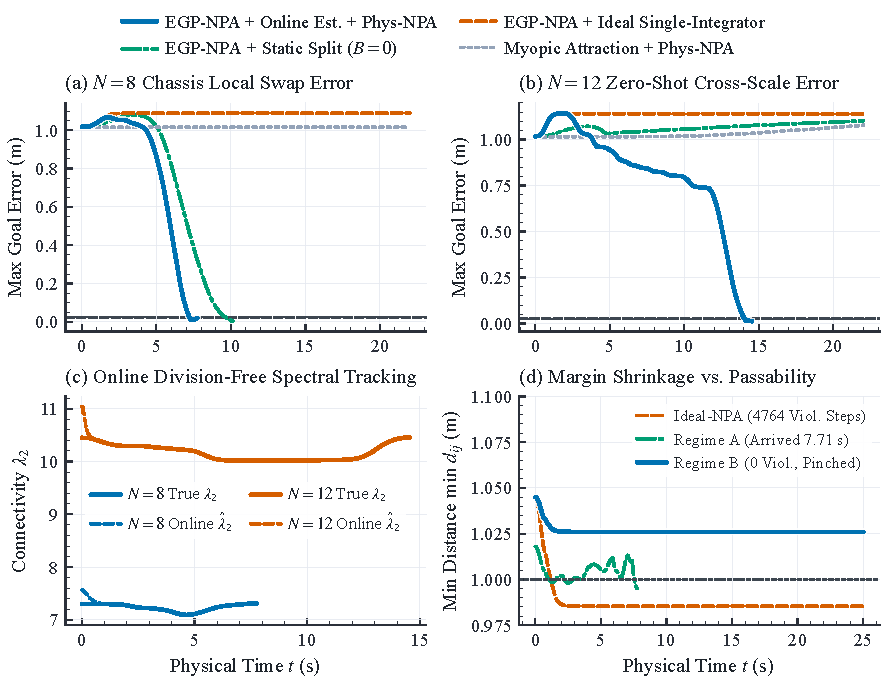
\includegraphics[width=\textwidth]{figures_en/fig6_mujoco_verification.pdf}
 \caption{Full-stack \texttt{MuJoCo} second-order omnidirectional chassis verification combining EGP-NPA, online division-free spectral estimation, and closed-neighborhood NPA. (a)--(b) Maximum goal error on $N=8$ and $N=12$ local swap tasks under Regime~A; (c) real-time $\hat{\lambda}_2(t)$ tracking by the division-free spectral estimator; (d) trade-off between minimum inter-robot clearance $\min d_{ij}(t)$ and channel passability across Ideal-NPA, Regime~A, and Regime~B.}
 \label{fig:mujoco}
\end{figure*}

\begin{theorem}[Critical Channel Pinch-Off Under Physical Margin Shrinkage]\label{thm:passability-tradeoff}
Consider $N$ robots swapping positions on a triangular lattice with initial spacing $S>\ds$, where outer neighbors $j,m$ can open a maximum lateral aperture $d_{jm}^{\max}$. Under physical safety margin shrinkage $\ds^{\mathrm{phys}}=\ds+\Delta d_{\mathrm{phys}}$ ($\mathcal S^{\mathrm{phys}}=\{\bp:\min_{a<b}d_{ab}\ge\ds+\Delta d_{\mathrm{phys}}\}$):
\begin{enumerate}
 \item \textbf{Static initial feasibility:} $\bp(0)\in\operatorname{int}(\mathcal S^{\mathrm{phys}})\Longleftrightarrow \Delta d_{\mathrm{phys}}<S-\ds$.
 \item \textbf{Three-body topological channel pinch-off:} For two counter-crossing robots $i_1,i_2$ passing simultaneously between $j$ and $m$, maintaining pairwise distances $\ge\ds^{\mathrm{phys}}$ at the symmetric midpoint requires a contact rhombus of side length $\ge\ds^{\mathrm{phys}}$, demanding a minimum lateral aperture $d_{jm}^{\mathrm{req}}(\Delta d_{\mathrm{phys}})=\sqrt{3}(\ds+\Delta d_{\mathrm{phys}})$. Whenever $\Delta d_{\mathrm{phys}}>d_{jm}^{\max}/\sqrt{3}-\ds$, the passage undergoes topological pinch-off in $\mathcal S^{\mathrm{phys}}$, disconnecting the initial and target configurations into separate path-connected components of $\mathcal S^{\mathrm{phys}}$.
\end{enumerate}
\end{theorem}
\begin{proof}
Claim (1) follows from $\min_{a<b}d_{ab}(0)=S$. For Claim (2), at the symmetric midpoint, $d_{i_1 i_2}\ge\ds^{\mathrm{phys}}$ and $d_{i_1 j},d_{i_1 m},d_{i_2 j},d_{i_2 m}\ge\ds^{\mathrm{phys}}$ imply $(d_{i_1 i_2}/2)^2+(d_{jm}/2)^2\ge(\ds^{\mathrm{phys}})^2\implies d_{jm}\ge\sqrt{3}(\ds+\Delta d_{\mathrm{phys}})$.
\end{proof}

Table~\ref{tab:mujoco} and Fig.~\ref{fig:mujoco} demonstrate both seamless estimator--policy coupling ($\hat\lambda_2$ RMSE $0.0255\sim 0.0438$ and $0$ connectivity violations across all $64$ runs) and the physical margin--passability trade-off predicted by Theorem~\ref{thm:passability-tradeoff}: under Regime~A ($S=1.018\ \mathrm m$), full-stack EGP-NPA achieves $3/4$ arrivals on $N=8$ and $1/4$ on $N=12$ (vs. $0/8$ for Myopic and Ideal-NPA), whereas enforcing $\Delta d_{\mathrm{phys}}=0.028\ \mathrm m$ under Regime~B eliminates soft-boundary grazing ($0$ violations on $7/8$ tasks) at the cost of pinching off the three-body swap channels.

\section{Conclusion}\label{sec:conclusion}

This paper presented the Envelope Equivariant Graph Policy with Neighborhood Proximal Allocation (EGP-NPA) framework for cooperative deadlock resolution of multi-robot systems subject to coupled collision avoidance and global algebraic connectivity constraints. First, an exact rational second-order KKT certificate on a seven-robot symmetric contact configuration (Theorem~\ref{thm:seven-kkt}) proved that safe and spectrally connected reachability does not imply reachability under myopic error-monotone safety filters, identifying lateral symmetry-breaking drive and dynamic quota-driven neighbor yielding as necessary and sufficient conditions for deadlock resolution. Second, we developed an $\mathrm{SO}(2)\ltimes\mathbb R^2$ and permutation-equivariant one-hop GNN residual nominal policy (Proposition~\ref{prop:equivariance}), proving why preserving $\mathrm{SO}(2)$ chiral orientation over full $\mathrm{O}(2)$ reflection equivariance is essential to prevent zero tangential output on symmetric head-on encounters. Third, we established anytime continuous-time safety invariance (Proposition~\ref{prop:safety}), derived the closed-form solution for cooperative unfreezing of stationary neighbors via dynamic quota transfer (Proposition~\ref{prop:unfreeze}), and proved first-order $\mathcal O(\norm{\be_k}_2)$ residual suppression and goal equilibrium recovery under the stateless one-hop completion envelope $\rho_{i,k}$ (Proposition~\ref{prop:envelope}). Across $96$ training-scale and zero-shot cross-scale benchmarks and $48$ independent holdout instances, EGP-NPA achieved $100\%$ safe arrival and zero safety violations—significantly outperforming shield-consistent safe MARL ($53.1\%,p=6.1\times 10^{-5}$), decentralized static-CBF shielded GNN ($3.1\%,p=9.3\times 10^{-10}$), primal-dual MAPPO-Lagrangian ($0\%$ violation-free arrival), tangential circulation heuristics ($40.6\%,p=3.8\times 10^{-6}$), and myopic CBF filtering ($15.6\%,p=1.5\times 10^{-8}$)—while second-order \texttt{MuJoCo} simulations with online division-free spectral estimation validated full-stack integration and characterized the physical safety-margin versus channel-passability trade-off (Theorem~\ref{thm:passability-tradeoff}). Future work will incorporate multi-scale boundary-clearance features and multi-seed curriculum training on larger lattices, as well as extensions to nonholonomic and field-of-view-constrained multi-robot teams.


\bibliographystyle{IEEEtran}
\bibliography{references}

\end{document}
